\documentclass[journal=mamobx,manuscript=article]{achemso}


\usepackage[version=3]{mhchem}
\usepackage{amsmath}
\usepackage{xcolor}
\usepackage{amsfonts}
\usepackage{amssymb}
\usepackage{graphicx}
\usepackage[english]{babel}
\usepackage{chemfig}
\newcommand{\species}[1]{\textit{#1} sp.}
\usepackage{subcaption}
\usepackage{cancel}
\usepackage{multicol}
\newcommand*\mycommand[1]{\texttt{\emph{#1}}}
\newcommand{\leng}{\mathcal{L}}





%%%%%%%%%%%%%%%%%%%%%%%%%%%%%%%%%%%%%%%%%%%%%%%%%%%%%%%%%%%%%%%%%%%%%
%% If issues arise when submitting your manuscript, you may want to
%% un-comment the next line.  This provides information on the
%% version of every file you have used.
%%%%%%%%%%%%%%%%%%%%%%%%%%%%%%%%%%%%%%%%%%%%%%%%%%%%%%%%%%%%%%%%%%%%%
%%\listfiles





\author{Sperydon Koumarianos}
\affiliation{Department of Physics and Astronomy, York University, Toronto, ON, Canada. M3J 1P3} 
\alsoaffiliation{Department of Mathematics and Statistics, York University, Toronto, ON, Canada.  M3J 1P3}

 
\author{Rohith Kaiyum}
\affiliation{Department of Physics and Astronomy, York University, Toronto, ON, Canada. M3J 1P3} 

\author{Christopher J. Barrett}
\affiliation{Department of Chemistry, McGill University, Montreal, QC, Canada.  H3A 2K6}
\alsoaffiliation{Department of Physics and Astronomy, York University, Toronto, ON, Canada. M3J 1P3} 

\author{Neal Madras}
\affiliation{Department of Mathematics and Statistics, York University, Toronto, ON, Canada.  M3J 1P3}

\author{Ozzy Mermut}
\affiliation{Department of Physics and Astronomy, York University, Toronto, ON, Canada. M3J 1P3}
\email{omermut@yorku.ca}


\title[An \textsf{achemso} demo]{Theory and Experiment of Chain Length Effects on the Adsorption of Polyelectrolytes onto Spherical Particles:  The Long and the Short of It}

\keywords{American Chemical Society, \LaTeX}

\begin{document}

\begin{abstract}

We study here the role of polyelectrolyte chain length, that is number of repeat units (mers), in the competitive adsorption of a simple model polyanion, poly(acrylic acid), onto 85nm spherical silica particles capped with a model polycation, poly(allylamine hydrochloride). Performing fluorescence spectroscopy experiments, we measured chain-length dependence of dilute aqueous polyelectrolyte adsorption, at full surface coverage, onto an oppositely charged polyelectrolyte overtop spherical silica nanoparticles ($10^{-3}$ g/L). Preferential adsorption was determined by comparing the characteristic fluorescence intensities  of the  two  fluorophore-labeled  and narrowly disperse polyacrylic acid samples (NMA-PAA\textsubscript{450K}  and Dan-PAA\textsubscript{2K}) of 450K- and 2K- molecular weight (6250- and 28-mers), respectively. To compare and validate experimental results, a lattice model was developed for computing the probabilities of the different arrangements of two polymer chain lengths of polyacrylic  acid  on  the  surface  of  the  silica  nanosphere. We then determined which numbers of long and short adsorbed chains corresponded to the most configurations in our model. Both spectroscopic experiment results and the combinatorial model demonstrated that there is an entropic preference for complete adsorption of the longer 450K polyacrylic acid chain  vs  2K. This study provides insights on entropy driven chain-length  dependence of polyelectrolyte adsorption onto spherical nanoparticle surfaces for directing and optimizing their  layer-by-layer self-assembly in organic films.


\end{abstract}
\newpage
\section{1. Introduction}  %2
    \label{sec-intro}
Understanding the adsorption behavior of charged self-assembling macromolecules onto surfaces is important in various applications governed by interfacial phenomena, soft matter film fabrication, surface functionalization, and stabilization of colloidal suspensions of inorganic nanoparticles.\cite{Dorris2011}  Most recently, such electrostatic self-assembly absorption onto small-curvature micro- or nanoparticles has received much interest for tissue scaffolds and various other biomedical engineering applications, where the soft, loopy hydrophylic polymer layers have been investigated as `bio-camouflage' coatings to improve bio-compatibility at these interfaces.\cite{Landry2019} 
Towards this interest in developing such new molecular soft coating architectures that cover a wide range of length scales, various methods to self-assemble and organize polymers on surfaces continue to be explored, from covalent attachment techniques\cite{doi:10.1002/ijch.199600050,B210143M,doi:10.1002/masy.200450305} to soft non-covalent physisorption approaches.\cite{Chen1992,Serizawa2002} An especially promising technique for preparing polymer thin films uses electrostatic ionic interactions between oppositely charged polyelectrolytes to assemble multilayer organic films on a wide variety of inorganic surfaces.  This method of polyelectrolyte assembly is now widely used in broad areas of materials science.\cite{Decher1997}  
Polyelectrolyte multilayer films (PEMs) are built-up layer-by-layer (LBL) by alternating adsorption of polycations and polyanions from aqueous solution onto a surface,\cite{Decher2006} a fabrication process that is experimentally simple, and versatile with respect to the surfaces, topologies, and materials that can be coated.  
Furthermore, optimization of industrial applications of functional PEMs, for example as biomedical materials, have provided impetus to explore in detail experimentally the nature of the driving forces governing LBL formation, specifically the interactions between adsorbed polyelectrolyte layers, and the influence of basic polyelectrolyte properties on LBL self-assembly of polyelectrolyte coatings such as charge, flexibility, and chain length (molecular weight).

Key to controlling the LBL process and the multilayer film properties is understanding parameters which govern the adsorption of polyions from solution onto surfaces containing oppositely charged polymers.\cite{Schonhoff2003}  
Extensive early theoretical work regarding the adsorption criteria for neutral polymers onto surfaces has previously been attempted, which has provided both quantitative predictions\cite{Fleer1982,Baumgartner1991} and basic scaling relations.\cite{DeGennes1976,Alexander1977}  
For example, theoretical calculations for neutral polymers have shown that its adsorption is dependent on the chain length,\cite{Stuart1980} and these results have been encouraged by early experiments.\cite{Stuart1980,Felter1970}  
More recent theoretical attempts to model polyelectrolyte adsorption have reaffirmed the challenge in generalizing the treatment addressing the formation of PEMs,\cite{Szilagyi2014} illustrating that these assemblies are often strongly non-equilibrium in nature.  In addition to accounting for complex electrostatic forces (i.e.\ by incorporating Debye-H\"uckel length-scales for polyions whose charge density can be highly sensitive to the local ionic strength at assembly),\cite{Chatellier1996} one must also consider this non-equilibrium adsorption and role of adsorption/redissolution kinetics, which are important to successfully capture the build-up of PEMs.\cite{Kovacevic2002} 
Hampering all of these first theoretical treatments was a lack of direct experimental verification as a guide to the modeling, as the various predictions provided generally govern adsorption thicknesses of a single molecular layer, of Angstroms to 1 or 2 nm at most, which required atomically flat surfaces experimentally to observe, and advanced techniques to measure the properties of soft, wet polyelectrolyte single molecular layers adsorbed.  Adding to this challenge was the desire to measure these molecular layers in the aqueous environment in which they were assembled and for biomedical applications in which they will be applied, and especially intrinsic properties of the polyelectrolyte chains themselves such as chain length (molecular weight), or coil properties (loops, tails), that become effectively indistinguishable in the 2D ensembles of coating coverage with PEMs.   Since the early theoretical attempts however, more sensitive experiments have been developed and reported to indeed make some of these measurements, to provide important feedback to the models regarding PEM coating thickness 
\textit{in situ} in a wet aqueous environment, surface charge, and the nature and geometry of the soft bonding interactions.\cite{Smith2004,Tanchak2004,Harroun2005,Burke2005,Tanchak2006}   Experimental confirmation of the length of the chains (molecular weight) of the adsorbed polymer proved to be an especially elusive problem to solve, but more recent attempts to transition from flat surfaces to high surface-to-volume ratio systems of PEMs adsorbed onto high-curvature inorganic particles, have permitted power bulk spectroscopic techniques to be employed, such as NMR and zeta potential electrophoresis,\cite{Burke2003,Mermut2003,Smith2004,Smith2003} providing an experimental roadmap to potential approaches for direct measurement of the molecular weight (chain length) of single adsorbed polyelectrolyte chains on analogous curved surfaces.  Previous experiments have been conducted on the effect of low molecular weights on the construction of polyelectrolyte multilayers observed by ellipsometry and optical waveguide examining polyelectrolyte stripping, and the production of a stable solution dispersion of polyelectrolyte complex.\cite{Sui2003}  An effect of chain length has also been reported on the formation of complex biological multilayered assemblies of alternating globular proteins (albumin, IgG) and linear strong polyanions (poly(styrenesulfonate), dextran sulfate, heparin) but only at pH below the isoelectric point of the protein.\cite{Houska2004}  These studies allude to the importance of studies, at the single layer level, both experimental and theory to examine a single layer adsorption as a function of polyelectrolyte chain length.

In this study, we examine the role of polyelectrolyte chain length (more specifically, number of repeat units, mers) in an individual adsorption layer of a simple model polyanion, poly(acrylic acid) onto silica particles capped with a model polycation, poly(allylamine hydrochloride).  Such studies of the adsorption behavior of charged macromolecules are also important in order to understand more generally various relevant biological surface and biointerface phenomena that cannot easily be probed experimentally by traditional techniques.  For example, the adhesion of bacterial cells to solid surfaces (governed by electrostatic, van der Waals, and Lewis acid-base interactions) is often largely affected by cell-surface polymers, such as lipopolysaccharides,\cite{Jucker1997} where   the affinity and reversibility of this adsorption process have been found to depend significantly on the molar mass of the cell surface polysaccharides involved in the adhesion.\cite{Jucker1997}  
Recently, it has also been found that strong electrostatic interactions lead to entropically favorable binding of charged peptides in the formation of a self-assembled monolayer adsorbed onto a gold surface.\cite{Sprenger2016} 
Specifically, we study here the role of polyelectrolyte chain length in the competitive adsorption of a simple model polyanion, poly(acrylic acid), onto spherical silica particles capped with a model polycation, poly(allylamine hydrochloride). Theoretical calculations for neutral polymers show that there is preferential adsorption that is dependent on the chain length, i.e.\ the number of mers, of the adsorbing polymer. 
We have performed experiments to investigate preferential polyelectrolyte adsorption behavior. 
This was achieved by spectroscopic 
observation of chain-length dependence between two widely differing molecular weights of fluorescently-labeled PAA polyelectrolytes allowed to adsorb competitively onto an oppositely charged PAH polyelectrolytes covering a spherical silica nanoparticle surface in dilute aqueous solution. 
Preferential adsorption was confirmed by comparing the measured fluorescence intensities of the two fluorophore-labeled (NMA-PAA\textsubscript{450K}, and Dan-PAA\textsubscript{2K}) polyacrylic acid samples presented to the surfaces, representing long or short molecular weight chains of equal mers total, by measuring signals specific to the 450K and 2K chains, respectively. To validate these experimental results, a computational model was developed that examined the entropy probability between the different arrangements of two polymer length chains of polyacrylic acid on the surface of the silica nanoparticles. This was done by comparing every scenario of surface coverage, using the associated likelihood of its occurrence. 
Both spectroscopic experiment results and the combinatorial model demonstrated that when presented with an equal total number of mers (both short and long chains),
there is an entropic preference for complete adsorption of the longer 450K polyacrylic acid chain vs 2K. This study provides insights on entropy driven chain-length dependence in LBL assembly, enabling optimization of industrial processes and developments of polyelectrolyte membranes and coatings, and rationalizing previous experimental results that suggested an entropic preference for longer chains to adsorb over shorter chains.

\section{2. Methods}  %3
     \label{sec-methods}
     
\subsection{2.1 Experimental}  %3.1
    \label{sec-meth-exp}

\subsubsection{2.1.1. Materials}   %3.1.1
       \label{sec-materials}

We used poly(allylamine hydrochloride) (PAH) as received from Polysciences, Inc. Poly(acrylic acid sodium salt) (PAA) of two different molecular weights (M\textsubscript{W} 2K and 450K, corresponding to 28 and

6250 mers respectively) Sigma-Aldrich and modified with fluorophores as described in section 2.1.2. 
The two different molecular weights of PAA were chosen based on the large difference in the average chain length (i.e.\ by greater than 2 orders of magnitude).  Furthermore, dynamic light scattering characterization (Brookhaven BI9000; Thorn EMI Electron B2FBK RFI photomultiplier tube; Coherent Technologies Compass 315M-150 laser) of the low and high molecular weight PAA, showed very little overlap in the histograms of the hydrodynamic radius of the polymers under the solution conditions used for the adsorption experiments.  Chemical structures for the polycation, unmodified polyanion, 
and the two labeled poly(acrylic acids) are presented in Figure \ref{figure 1}.  We prepared aqueous polyelectrolyte solutions of concentration $10^{-2}\,$M (based on the molecular weight of repeat units) using 18.2 M$\Omega\cdot$cm resistivity Millipore Milli-Q water and the adsorption experiments were done in the presence of 1 M NaCl.

\begin{figure}[H]
    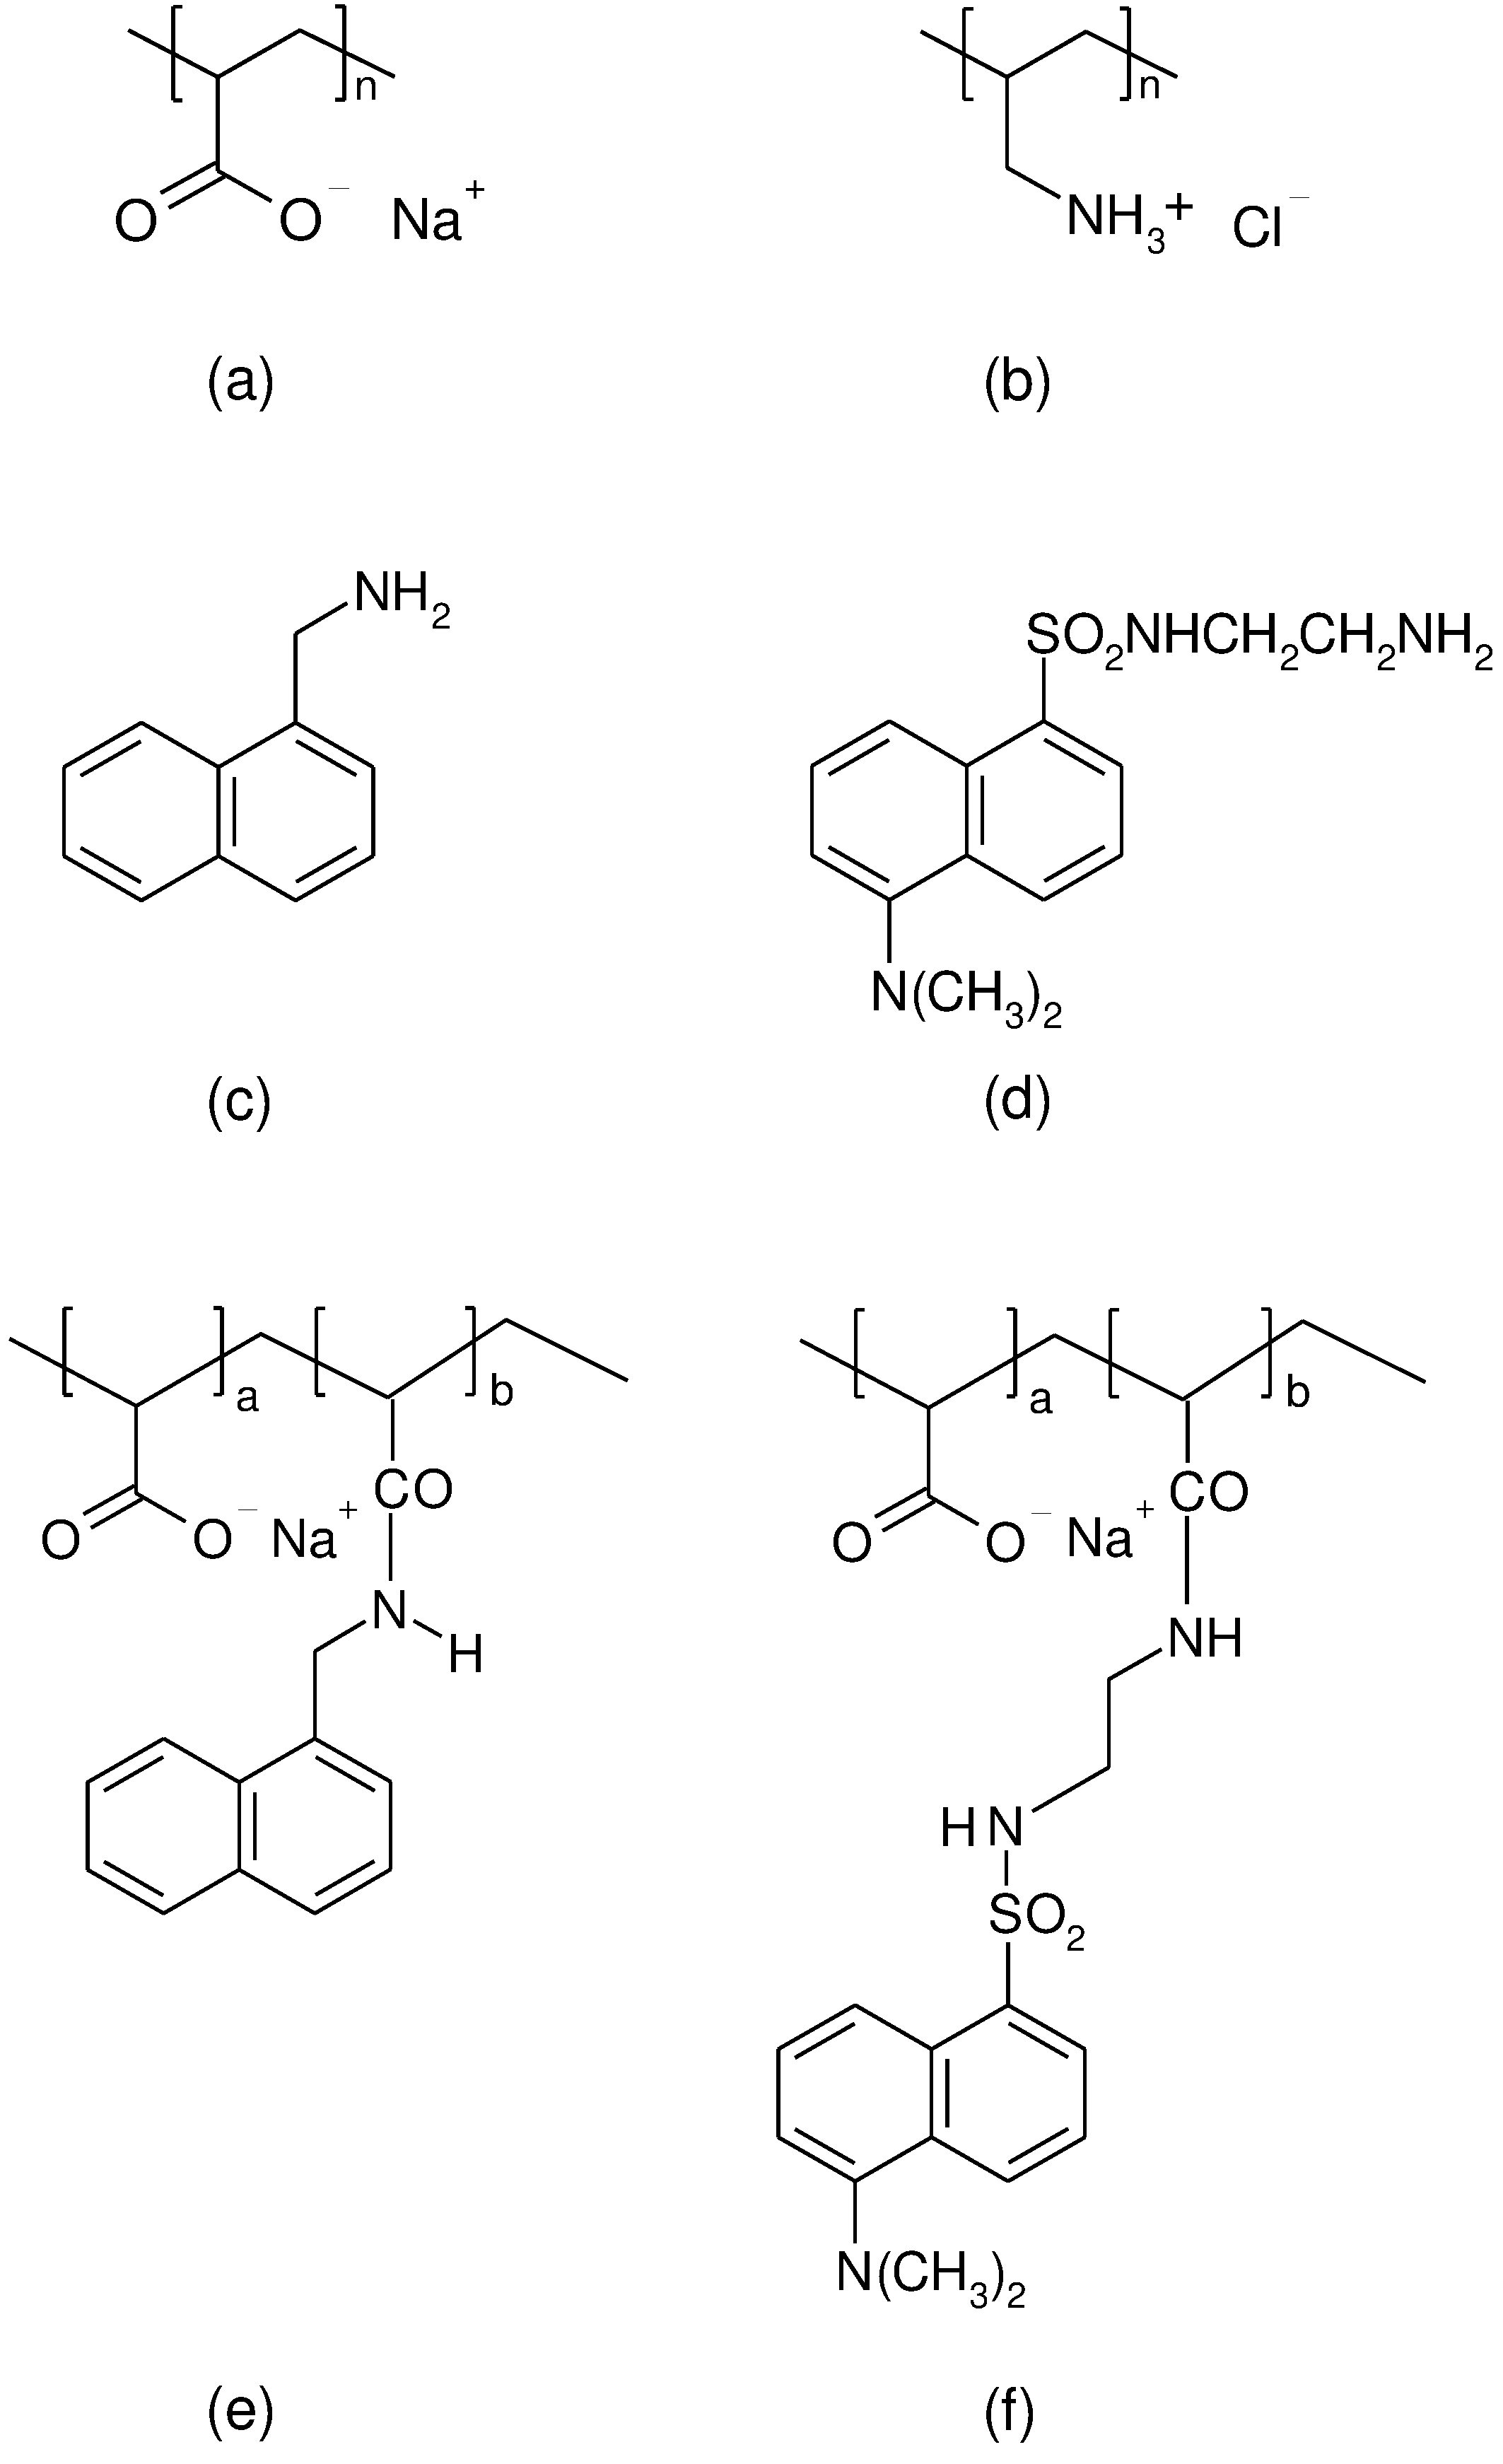
\includegraphics[scale=0.25]{allChems_30apr2020.pdf}
    \caption{Structures of the polyelectrolytes used are: a. poly(allylamine hydrochloride), and b. poly(acrylic acid sodium salt).  Fluorophores used to label the polyanion are: c. 1-naphthylmethylamine, and d. dansyl ethylenediamine (D112).  Structures of labeled poly(acrylic acid) are: e. NMA-PAA\textsubscript{450K}, and f. Dan-PAA\textsubscript{2K}. }
    \label{figure 1}
\end{figure}


Two naphthalene-based fluorophores with amine functional groups, 5-dimethylaminonaphthalene-1-(N-(2-aminoethyl))sulfonamide (also known as dansyl ethylenediamine), and 1-naphthylmethylamine were purchased from Molecular Probes, and Sigma-Aldrich respectively.  Our adsorbing surface was colloidal silica of 70-100 nm in diameter, received from Nissan Chemical Industries. The pH of the solutions was adjusted to a value of 9.0 using NaOH.  At pH = 9.0, we can observe the adsorption of strongly charged PAA onto a mostly weakly charged PAH surface (since PAH was first adsorbed onto the colloidal particles).

\subsubsection{2.1.2 Derivatization of PAA with Fluorophores}  %3.1.2
    \label{sec-derivPAA}

Through a method previously described, \cite{weber1954fluorescent,Anghel1998} partial conversion of the carboxylic acid units of the 2K and 450K PAA to amide derivatives (amidization) was achieved in two separate reactions as follows:  Inside a dry three-neck flask attached to a condenser, vacuum dried PAA (2.0 g) was mixed with an anhydrous solvent, 1-methylpyrrolidone (approximately 100 ml), in the presence of flowing nitrogen.  The mixture was stirred to allow for dissolution (in the case of 2K PAA) or additionally heated to $60^{\circ}$C for 2 hr (in the case of 450K) to promote dissolution.  In a dry and nitrogen-rinsed flask, the fluorophore (7.0 $\times$ $10^{-4}$ mol) was dissolved in some 1-methylpyrrolidone (approximately 5 ml) and injected into the PAA reaction pot.  Subsequently, dicyclohexylcarbodiimide (DCC, 8.0 $\times$ $10^{-4}$ mol), a coupling agent commonly used to promote amide formation was also injected into the reaction mixture upon dissolving in dry 1-methylpyrrolidone (approximately 5 ml).  The use of an aprotic solvent, 1-methylpyrrolidone, and DCC promotes the random covalent attachment of the hydrophobic fluorophores onto PAA.\cite{Anghel1998}  The final mixture was stirred in the dark at $60^{\circ}$C for 96 hr.  The reaction flask was then cooled in an ice bath, and concentrated NaOH was added dropwise to neutralize the solution, which resulted in precipitation of the sodium salt of the modified PAA.  The solid product was obtained by vacuum filtration and subsequently purified by twice precipitating an aqueous solution in methanol.  All solvents were removed to yield the final product by drying in a vacuum oven.

Both the unmodified and labeled PAA were characterized by $^{1}$H NMR (300 MHz Varian Mercury) performed in D$_2$O.  In the case of 1-naphthylmethylamine-labeled PAA (NMA-PAA$_{450K}$) $^1$H   spectrum analysis shows the expected ratio of naphthalene (7) and amide (1) protons at chemical shifts of 7-8 ppm while the alpha aromatic proton (1) appears at 4.7 ppm.  In unmodified PAA, only methylene protons from the backbone (1-2.3 ppm) appear in the $^1$H NMR spectrum.  The $^1$H NMR spectrum of dansyl ethylenediamine-labeled PAA (Dan-PAA$_{2K}$) also reveals the expected chemical shifts at 7.2-8.3 ppm from the aromatic protons of the fluorophore, and the $\beta$, $\gamma$ methylene protons (4) from the amide link at around 3.4 ppm.  Both UV-vis absorption (Varian Cary 300-Bio Spectrophotometer), and $^{1}$H NMR spectral analysis of the final product suggested little contamination of labeled PAA and the degree of modification was calculated by integration of the $^{1}$H NMR spectral peaks.  It was determined that PAA of 450K was 3.8 mol\% modified while 4 mol\% of the 2K PAA was labeled.  The degree of derivatization of PAA was kept at a low value to prevent interference from the hydrophobic fluorescent tags on the electrostatic adsorption of the polyelectrolyte.  Fluorescence intensity calibration plots at variable concentration of NMA-PAA\textsubscript{450K} and Dan-PAA\textsubscript{2K} were prepared using a FluoroMax-2 (Jobin Yvon-SPEX; slit width set to 2.5 cm). 

\subsubsection{2.1.3a Preliminary Adsorption of PAH onto Colloids}   %3.1.3a
    \label{sec-prelPAH}


An excess amount of the polycation layer, poly(allylamine hydrochloride), was first provided for adsorption onto colloidal SiO$_2$ according to the following standard protocol previously outlined for the preparation of PAH/PAA multilayers onto SiO$_2$.\cite{Burke2003}  In this protocol the polyelectrolyte adsorption conditions are set to a pH value of 9.0 and 1.0 M of NaCl was used to ensure highest coverage of the colloid with the polycation.  Colloids were dispersed in a polyelectrolyte solution for 30 min, followed by 1 h of centrifugation at 4500 rpm.  The supernatant is then removed and the colloids are washed three times with Millipore Milli-Q water (adjusted to pH = 9) to remove unadsorbed polymer.  Each wash step consists of 30 min of sonication (to expose colloids to wash solution while preventing aggregation), 1 h centrifugation, and finally extraction of the liquid.  

\subsubsection{2.1.3b Competitive Adsorption of PAA onto a PAH-Coated Surface}    %3.1.3b
    \label{sec-exp-compet}

The competitive adsorption of long (450K) versus short (2K) chains of PAA was examined by supplying in solution a stoichiometric surface coverage amount of each of Dan-PAA\textsubscript{2K} and NMA-PAA\textsubscript{450K} to 2.0 g/L of PAH-coated particles.  This required surface coverage amount of polyelectrolyte (3\,--\,5$\,\times \,10^{-4}$ M repeat units of each type of PAA) for 2.0 g/L of PAH-coated particles was determined from quantitative titrations of PAH/PAA-coated particles with poly(diallyldimethyl-ammonium chloride) (PDAC).\cite{Burke2003}   The molar concentration of labeled PAA necessary to cover the PAH surface (3-5 $\times$ $10^{-4}$ M for 2.0 g/L of particles) was obtained by converting the bare mass of titrant (PDAC) required to achieve charge overcompensation, and thus multilayer formation, to a molar surface coverage value (as determined by $\zeta$ potential measurements).\cite{Burke2003}   Specifically, this point refers to the mass of titrant at the initial plateau point after the half neutralization point in the titration curve (i.e.\ 0.05 g/L of PDAC for 2.0 g/L of coated particles).  Although this estimation of the surface coverage value is based on a titration experiment involving a different polyelectrolyte than that used in our experiment, it provides a reasonable approximation of the required coverage amount.  Furthermore, the titration experiment was performed under comparable solution conditions to our PAA adsorption study (1 mM NaCl and solution pH = 9) and in both cases the adsorbing polyelectrolyte is strongly charged.  Thus, assuming that the adsorption isotherms are comparable, the error in determining the surface coverage value is estimated to be in the range of the experimental uncertainty reported in the titration study, $\pm$ 9.6 \%.  We allowed 24 h to ensure coverage adsorption of the labeled PAA onto PAH since previous PAH/PAA multilayer studies have shown significant time-dependent adsorption at low polyelectrolyte concentrations (i.e.\ $<10^{-3}$ M).\cite{Mermut2003}

Figure \ref{figure 4} illustrates the two extreme outcomes for this competitive adsorption study.  Given an identical concentration of repeat units, the two extreme cases involve either sole preference for shorter chains of PAA (i.e.\ Case 1, where fluorescence is only detected from Dan-PAA\textsubscript{2K}) or the longer ones (i.e.\ Case 2, where only NMA-PAA\textsubscript{450K} fluorescence is observed).  A third possible scenario is that of an unbiased adsorption of both short and long chains, in which no change in the relative fluorescence signals would be expected before and after the adsorption. 

\begin{figure}[H]
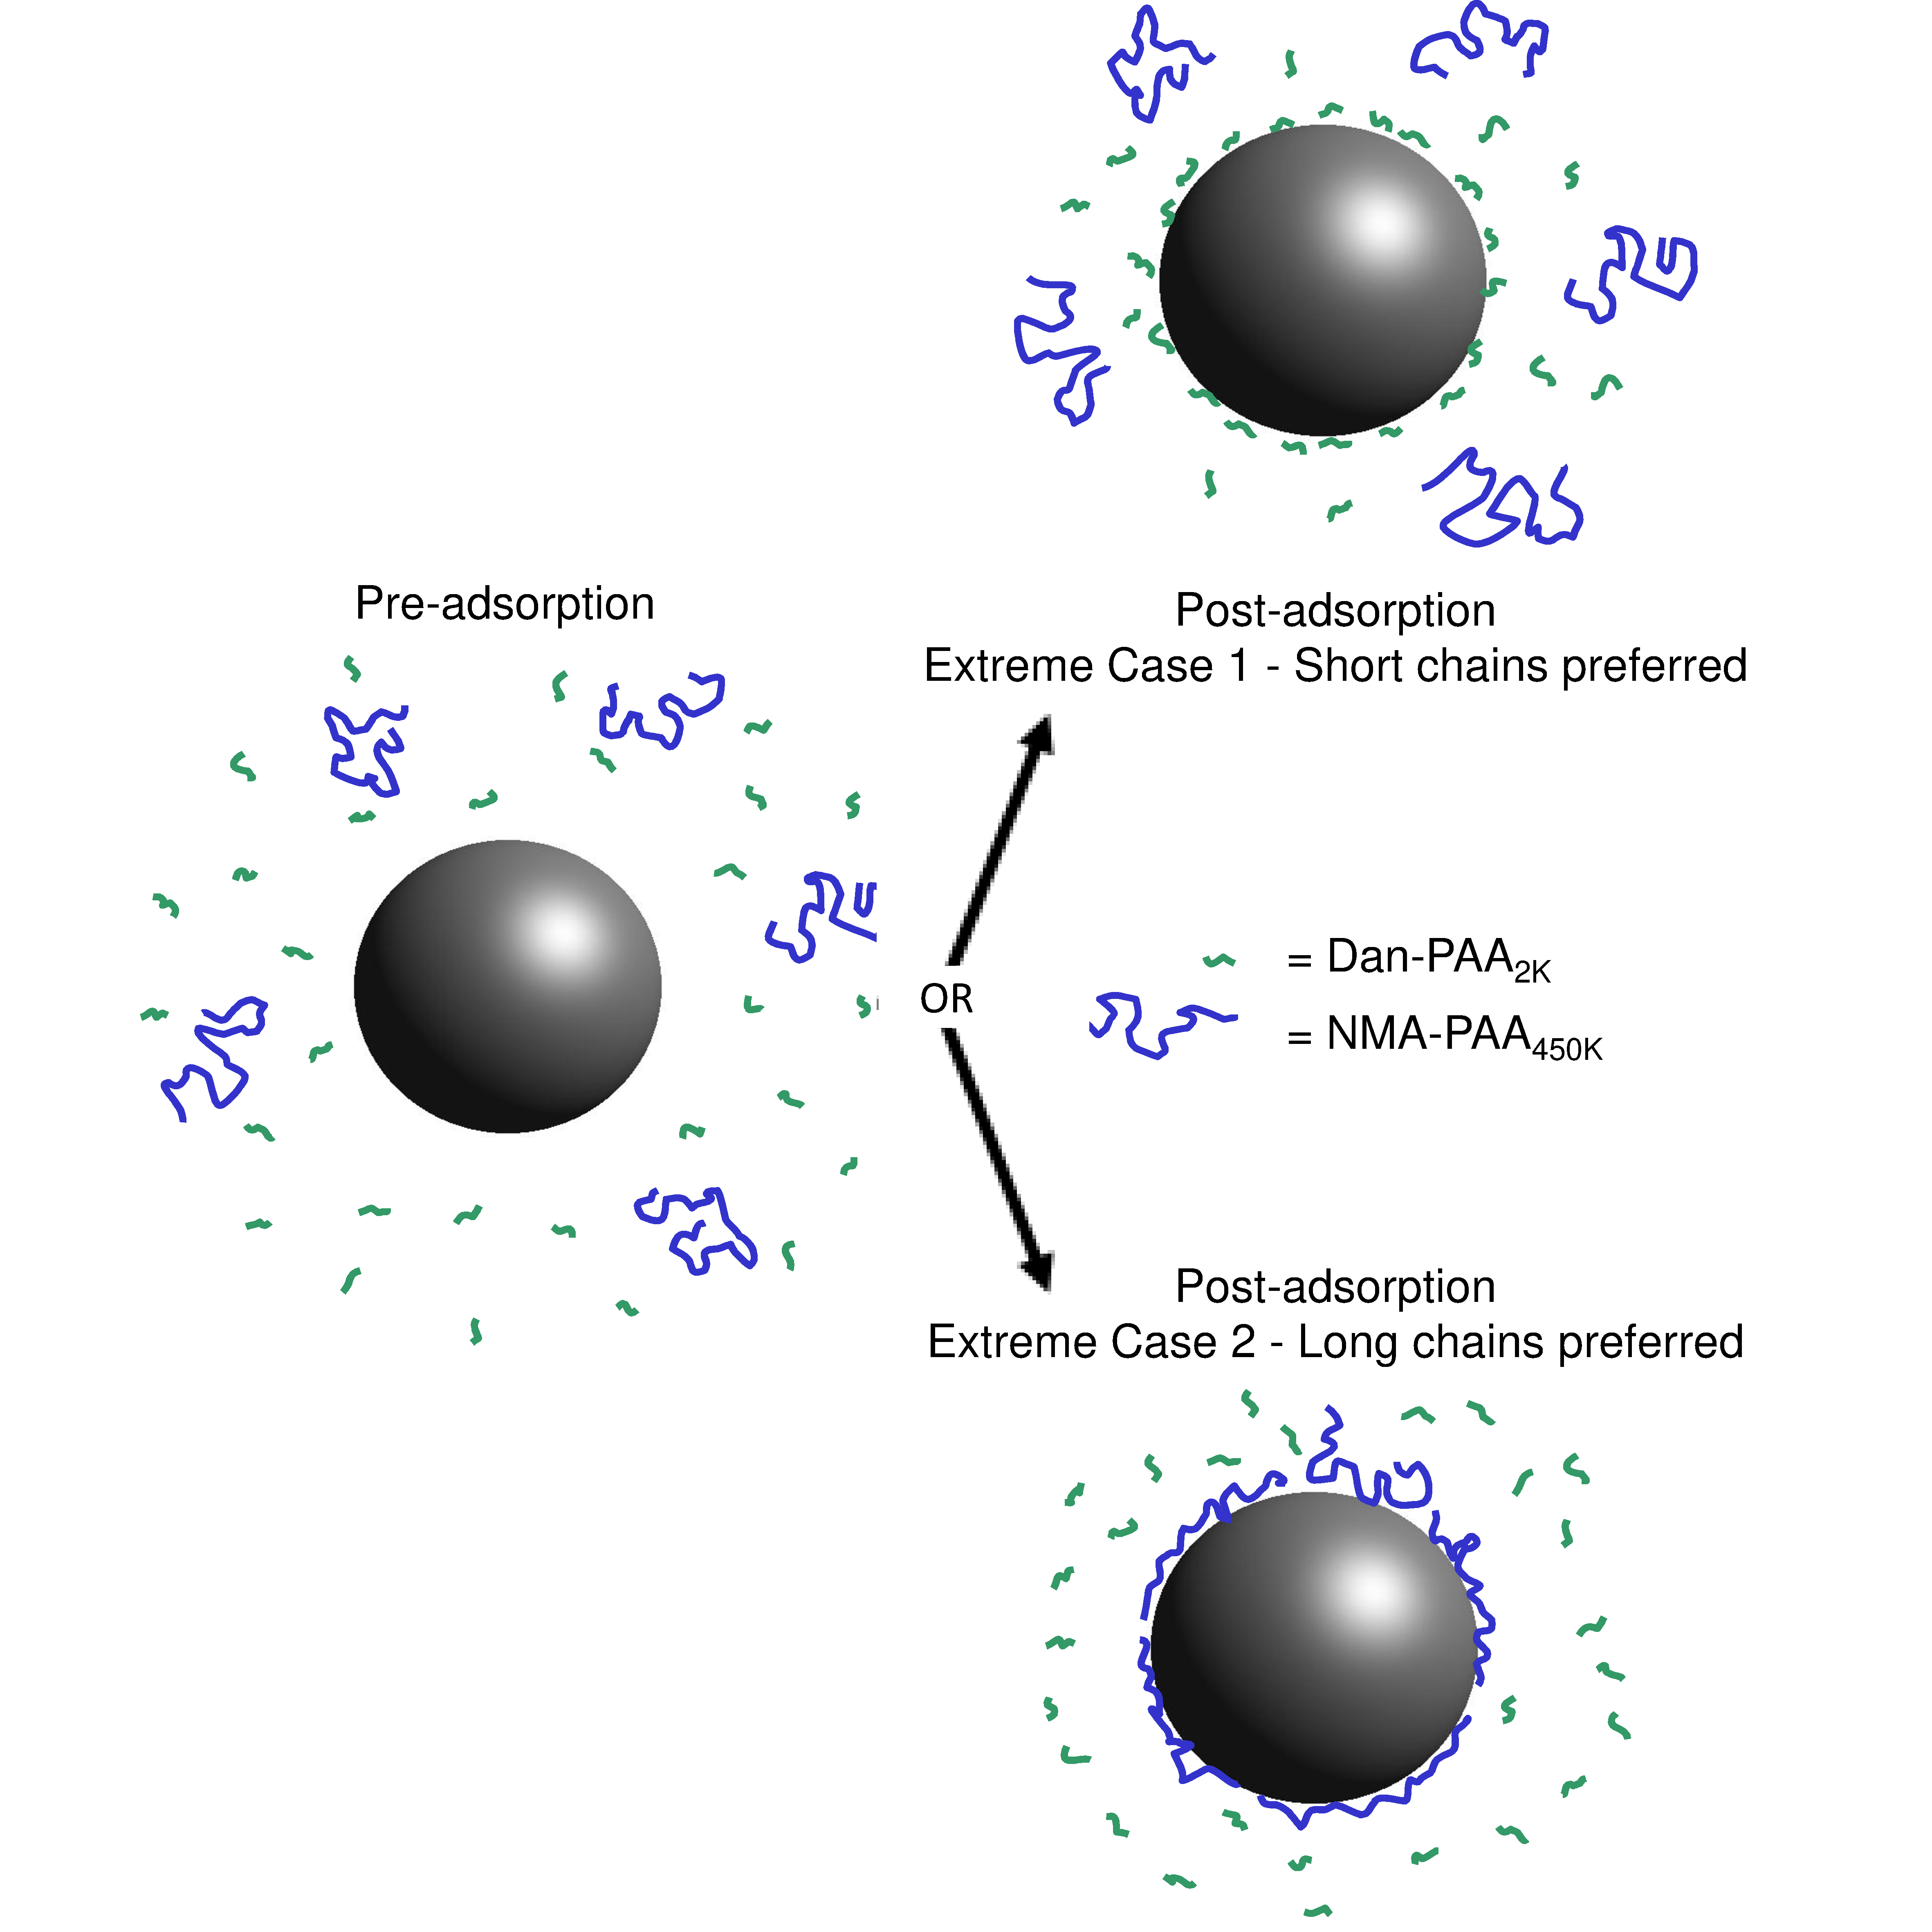
\includegraphics[scale=0.15]{Figure2.pdf}
\caption{Possible extreme results for the competitive adsorption experiment of PAA onto PAH-coated particles.  The two extreme cases show preference of the surface for only the short chains (emission only at $\lambda$\textsubscript{Em} = 550 nm from adsorbed Dan-PAA\textsubscript{2K}), or solely the long chains (emission only at $\lambda$\textsubscript{Em} = 550 nm from adsorbed NMA-PAA\textsubscript{450K}).  The third intermediate case (not shown) is that of indifferent adsorption.}
\label{figure 4}
\end{figure}


\subsubsection{2.2  Theoretical}   %3.2
    \label{sec-meth-theor}

\subsubsection{2.2.1 Development of Mean-Field lattice model}   %3.2.1
   \label{sec-devMF}

Here we develop a combinatorial approximation method
to model the preferential behavior of our system.
It has been recognized that long polymers are
preferentially adsorbed compared to shorter polymers,
due to the short polymer's greater gain of
translational entropy per monomer in three dimensions
as compared to two.\cite{Fleer1993} 
In light of the small number of polymers on each
spherical surface, we adapt existing methods to a
fully discrete setting to analyze this phenomenon in our
situation.  Our model maintains the property that the enthalpic energy is identical in both the scenarios of complete short or long-chain adsorption to the colloid surface, thereby reducing our problem
to one of pure 
combinatorial entropy. 

Our lattice model essentially addresses
the following issue.
Assume that both short and long polymers 
are dilute in the solvent, and that the 
surface of each colloidal sphere is completely covered 
by fully adsorbed polymer chains.  Then we 
can approximate the probability distribution of  fraction of the sphere's surface that is 
covered by short chains.  It turns out that this 
fraction is very likely to be small.
See  Equation (\ref{eq.jstar}) and discussion thereof for a more precise statement. 


We use the following lattice model to describe our experimental situation.  
Lattices appear in two ways:  (1) covering the surface of a sphere by a two-dimensional lattice, and
(2) filling space (the solvent) with a regular three-dimensional cubic lattice.  
The geometry of the lattices does not play a significant role.  
We let $q$ be the coordination number of the two-dimensional lattice 
(that is, each site on the surface has exactly $q$ neighboring sites).  We assume that 
the distance between lattice sites corresponds to the distance between adjacent monomers within a polymer.  
We assume that in equilibrium, every lattice site in the surface is covered by an adsorbed monomer.
We also assume that each polymer either has every monomer adsorbed onto the surface, or else has no adsorbed monomers (in the terminology of Fleer \textit{et al.},\cite{Fleer1993} the adsorbed chains
have no ``loops'' or ``tails'').

Our experiment had a large number $n_{sphere}$ of spheres in a solution of volume $V_{sol}$.  
To simplify 
our model and without changing the concentrations, we consider only a single sphere in a solution
of volume $V=V_{sol}/n_{sphere}$.  We refer to this as our model system (see Figure \ref{figure1volume}).
We view this small three-dimensional region of the solution in our model system as being filled by a 
cubic lattice.
Let $V_{latt}$ be the number of sites of the cubic 
lattice in our solution region of volume $V$.




 \begin{figure}[H] 
  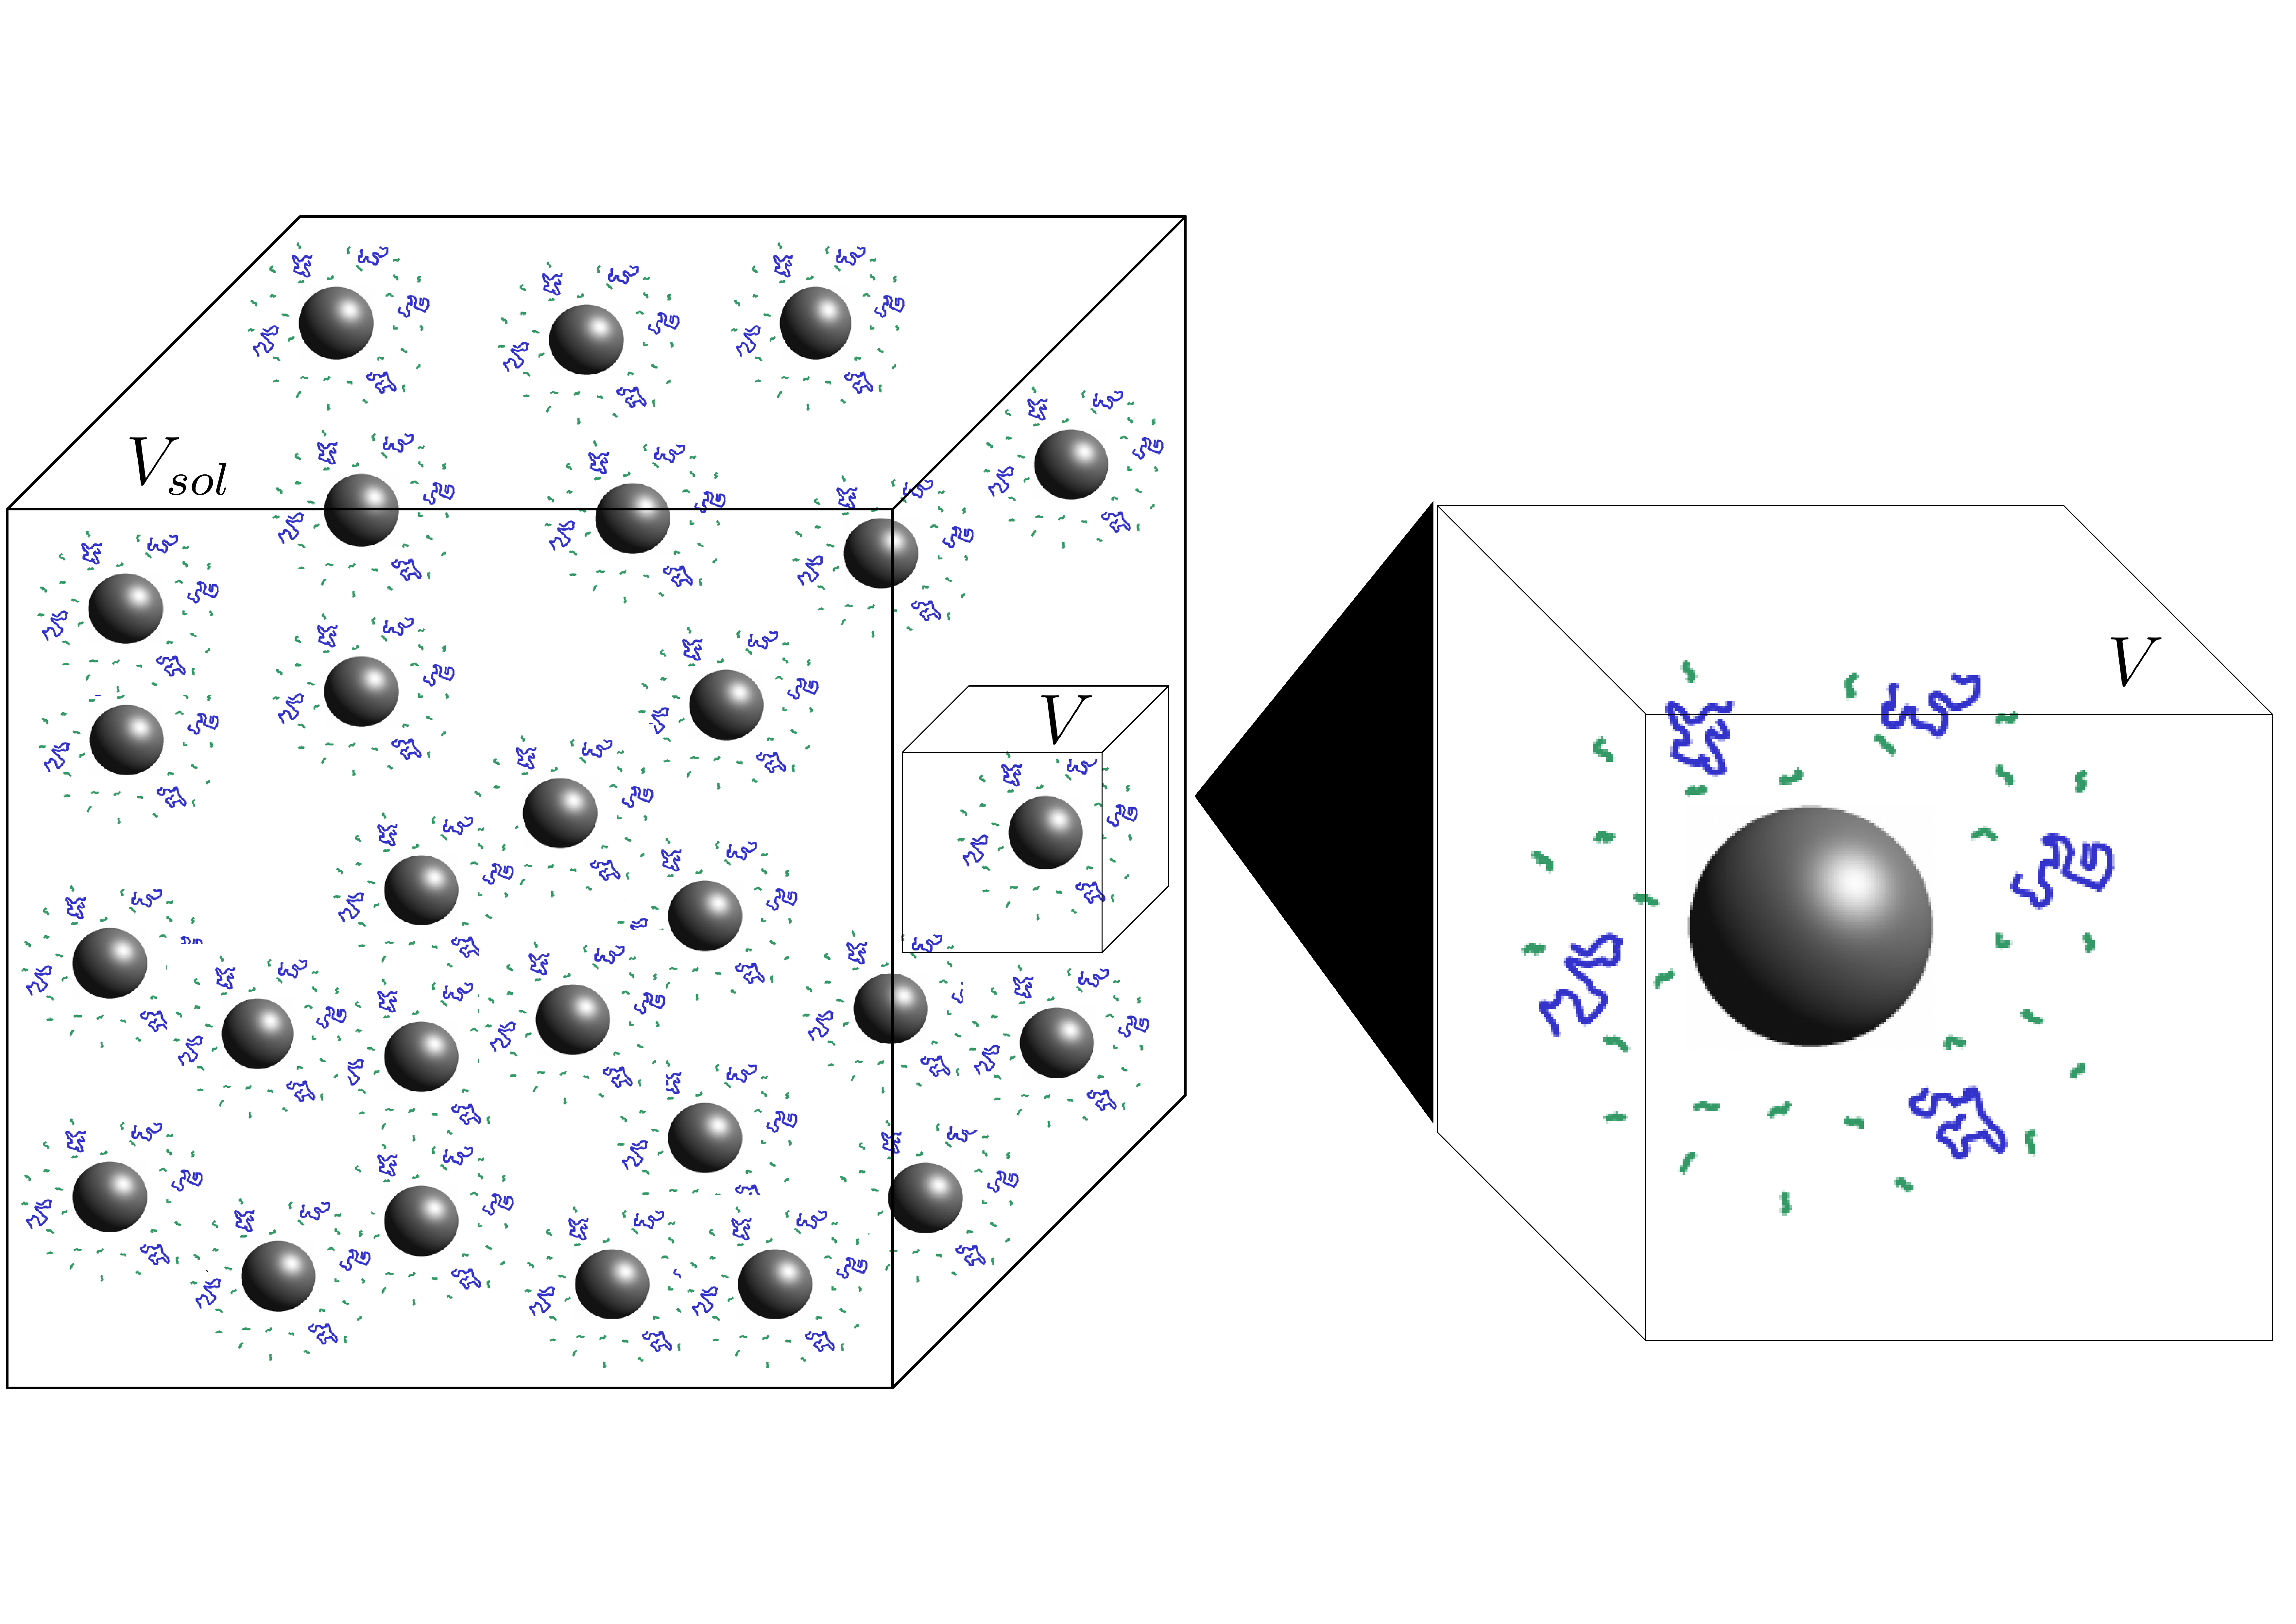
\includegraphics[scale=0.12]{Figure3.pdf}
\caption{Schematic of the model system (small box)
inside the full solution (large box). The full system
has volume $V_{sol}$ and contains many spheres. The model system has volume $V$, and contains one sphere (shown as the expansion on the right).}
\label{figure1volume}
\end{figure}




We model our polymer configurations as walks in lattice, but we use slightly different approaches for the solution and for the surface.
The difference is due to the fact that the polymers are dense on the surface but 
dilute in the solution.  We model the configurations of polymers in the solution as a collection of 
self-avoiding walks in the cubic lattice, with no interaction between walks (because of the dilute solution).
We view the polymers adsorbed densely on the surface lattice as non-reversed walks constrained to
be mutually and self-avoiding.  Since enumeration of
dense walks is difficult, we use a mean-field 
approximation of the Flory-Huggins type.\cite{Flory1953}

In our model system, we assume that the number of chains of each length is fixed.  
Let $n_S$ be the number of short chains
and let $n_L$ be the number long chains.
We also assume that each
short chain has the same number of monomers, 
which we denote $\leng_S$.  This ``length'' 
will equal the number of lattice sites (and be one
more than the number of bonds or steps) in each
walk that corresponds to a short chain.
Similarly, we assume that each long 
chain has $\leng_L$ monomers.
In the rest of this section, a ``configuration''
of our model system refers to a collection of $n_S$
walks of length $\leng_S$ and $n_L$ walks of length
$\leng_L$ (all disjoint), 
where each walk is either entirely in the 
surface lattice or else does not touch the surface
lattice, and the surface lattice is completely 
covered by walks.  
We write $\mathcal{E}$ for the 
set of all configurations of our model system.
This is a large but finite set.

Let $a$ be the maximum number of long chains that
can be fully adsorbed onto the surface lattice.
For each integer $j$ with $0\leq j\leq a$, let
$\mathcal{E}_j$ be the set of all configurations that have exactly $j$ long chains adsorbed 
onto the surface.  
Then the full space of configurations in our model,
$\mathcal{E}$, is equal to 
$\cup_{j=0}^a {\mathcal{E}_j}$. 

Since the only energy in this model comes from the adsorption contacts between monomer and surface,
and since every configuration in $\mathcal{E}$ has the same number of such contacts
(namely, the number of sites in the surface lattice),
we see that every configuration of $\mathcal{E}$ has exactly the same energy.
Therefore, according to the Boltzmann distribution, every configuration in $\mathcal{E}$ is equally
likely. Thus to calculate the probability of an event, we can simply count the configurations associated with the event and divide by the total number of configurations.
Specifically, denoting the number of configurations in a set $\mathcal{A}$ by $|\mathcal{A}|$, we see that
the probability that exactly $j$ long polymers are adsorbed is $\frac{|\mathcal{E}_j|}{|\mathcal{E}|}$,
for each $j=0,1,\ldots,a$.

Thus, to find the most likely number of long chains %(and $W$-mers (short-chains))
that are adsorbed onto the sphere, we need to 
find which of the sets $\mathcal{E}_j$ is largest.
Our goal is to show that there is an integer value $j^*$
such that
\begin{equation}
    \label{eq.EEcomp}
  |\mathcal{E}_0| \;<\; |\mathcal{E}_1|\; < \; 
 \cdots\; < \; 
  |\mathcal{E}_{j^*-1}|\; < \;|\mathcal{E}_{j^*}|\; >
    \; |\mathcal{E}_{j^*+1}| \;>\; \cdots \; > \; |\mathcal{E}_a|\,,
\end{equation}
and that $j^*$ is approximated by Equation (\ref{eq.jstar}) below.  
This value $j^*$ is the most likely
number of long chains to be adsorbed.


\subsubsection{2.2.2 Calculating the Most Probable Outcome}   %3.2.2
    \label{sec-calcMPO}

We now wish to estimate the size of each set $\mathcal{E}_j$ ($j=0,1,\ldots,a$), in order to  determine which set is the largest.  
As explained above, this corresponds to finding the most probable number of 
long polymers that are adsorbed in the experimental system. 

Recall that our model system has $n_S$ short 
polymers of length $\leng_S$ and $n_L$ long polymers
of length $\leng_L$.  
Let $S_{latt}$ be the number of lattice sites on 
the surface of one sphere.  Then $a$, which we
defined to be the maximum
number of long polymers that can be (fully)
adsorbed onto the surface of a sphere, is 
\begin{equation}
  \label{eq.aequal}
     a  \;=\;  \frac{S_{latt}}{\leng_L} \,.
\end{equation}
We assume that the right-hand side of this equation is an integer.  

It is convenient to define the quantity $n$ by \begin{equation}
   \label{eq.ndefn}
    n\;=\;\leng_L/\leng_S  \,,  \hspace{6mm}\hbox{i.e.}
     \hspace{5mm}  \leng_L  \;=\;  n\leng_S \,,
\end{equation}
so that
long polymers are $n$ times the size of the short ones.
It follows that the maximum number of short polymers
that can be adsorbed onto a sphere's surface is $na$.
To make the total %mass
number of mers the same for each
of the two sizes of polymers in our system,
we can assume that $n_S \,=\, n\cdot n_L$.  However, we do not really use this relation; it is enough that $n_S$ and $n\cdot n_L$
are of similar orders of magnitude.



As mentioned in Section 2.2.1, we model the configuration of a single  polymer in a dilute solution by a self-avoiding walk (SAW) in a lattice, which is a path in the lattice that does not visit any site more than once.

For each positive integer $\ell$, let $c_{\ell}$ be
the number of SAWs that start from a specified site of the simple cubic lattice and visit a total of $\ell$ sites (including the starting site).
Then $c_{\ell}$ exhibits the asymptotic
behavior\cite{Madras2013} 
\begin{equation}
    \label{eq.sawscale}
       c_{\ell}  \;\sim  \;  A_3 \, {\ell}^{\gamma_3-1}  \mu_3^{\ell}    \hspace{5mm}\hbox{as $\ell\rightarrow\infty$}.
\end{equation}
Here $\mu_3$ and $A_3$ depend on the choice of lattice, but $\gamma_3$ is a universal critical exponent
that is the same for all three-dimensional lattices.  
For the simple cubic lattice, 
their values are known to be approximately \cite{Chen2002,Madras2013}
\begin{equation}
   \label{eq.gammas}   \mu_3 \;=\;  4.684, \hspace{5mm}
        A_3 \;=\;  0.2573,    \hspace{5mm}\hbox{and}\hspace{5mm}
   \gamma_3 \;=\;  1.162 \,.  %1.205/4.683 \;=\;  \,.
\end{equation}
(Chen and Lin\cite{Chen2002} used the 
number of SAWs with $\ell$ \textit{steps} (i.e.\ $\ell+1$ \textit{sites}), which we write  $c_{\ell+1}=(A_3\mu_3)\ell^{\gamma_3-1}\mu_3^{\ell}$; 
they obtained $A_3\mu_3=1.205$.)
Since the number of sites in the lattice corresponding to the region of solution is $V_{latt}$, 
we have $V_{latt}c_{\ell}$ ways to place a polymer of size ${\ell}$.  As we are neglecting the
possibility of overlapping polymers in the dilute solution, it follows that the number of ways to 
place $N$ indistinguishable $\ell$-mers is 
\begin{equation}
  \label{eq.Npoly}
   \frac{(V_{latt}\,c_{\ell})^N}{N!}  \,.   
\end{equation}

 As described above, the integer variable $j$ 
 denotes the number of long chains that are adsorbed
 onto the sphere's surface ($0\leq j\leq a$).
 Given $j$, the number of $\leng_L$-mers (long-chains) in solution must be $n_L-j$; 
 the number of $\leng_S$-mers (short-chains) adsorbed on the surface must be $n(a-j)$ [because there are $S_{latt}=an\leng_S$ sites on the surface, all occupied, of which $j\leng_L$ are occupied by $\leng_L$-mers, leaving $S_{latt}-j\leng_L\,=\, an\leng_S-jn\leng_S$ to be  occupied by $\leng_S$-mers]; 
 and hence the number of $\leng_S$-mers (short-chains) in solution must be  $n_S-n(a-j)$.

Recalling Equations (\ref{eq.sawscale}) and 
(\ref{eq.Npoly}), we find that the number of configurations in $\mathcal{E}_j$ is
\begin{equation}
    |\mathcal{E}_j|  
      \; = \; \frac{ \Psi_L^{n_L-j} }{(n_L-j)!} \,
          \frac{ \Psi_S^{n_S-n(a-j)} }{(n_S-n(a-j))!} \,  G(j)
%           \frac{\tilde{w}_1\tilde{w}_2\cdots \tilde{w}_j}{j!}
 %                    \,   \frac{\tilde{u}_{nj+1}\tilde{u}_{nj+2}\cdots \tilde{u}_{an}}{(n(a-j))!}
        \label{eq.Yj}
\end{equation}
where 
\begin{equation}
    \label{eq.psidef}   
   \Psi_L\;=\;V_{latt} A_3 (\leng_L)^{\gamma_3-1} \mu_{3}^{\leng_L} \,,  
    \hspace{5mm} %\hbox{and} \hspace{5mm}
     \Psi_S \;=\; V_{latt}A_3{\leng_S}^{\gamma_3-1}\mu_3^{\leng_S} \,,
\end{equation}
and $G(j)$ is the number of ways to cover the surface
with $j$ $\leng_L$-mers and $n(a-j)$ $\leng_S$-mers.
The quantity $G(j)$ is difficult to compute, so we
approximate it using a mean field (Flory-Huggins) approach.  Details are given in the Supporting Information.

In section 1.1 of the Supporting Information, we show that
\begin{equation}
    \label{eq.Yratio2}
       \frac{|\mathcal{E}_{j+1}|}{|\mathcal{E}_j|} \; \approx \; \left( h(j)\right)^{n+o(n)}
       \hspace{5mm}\hbox{where}\hspace{5mm}
      h(j) \;=\;  \frac{ V_{latt}A_3\leng_S^{\gamma_3-1}(q-1)^2}{aq\leng_S} \,
          \frac{(a-j-\frac{1}{2})}{n_S-n(a-j-\frac{1}{2})}   \,.
\end{equation}
Observe that $h(j)$ is a  decreasing function of the integer variable $j$.
Let $j^*$ be the smallest value of $j$ for which 
$h(j)$ is less than 1. 
We now explain why Equation (\ref{eq.EEcomp}) holds 
for this choice of $j^*$, which in turn tells us that
$j^*$ is the most probable 
number of adsorbed long chains.
Firstly, for every $j\geq j^*$, we have $h(j)<1$, 
and thus Equation (\ref{eq.Yratio2}) shows that 
$|\mathcal{E}_{j+1}|/|\mathcal{E}_j|<1$, i.e.\ that 
$|\mathcal{E}_j|>|\mathcal{E}_{j+1}|$.  That is, $|\mathcal{E}_j|$ is decreasing in $j$ when $j\geq j^*$.  
Similarly, for $j<j^*$ we have $h(j)>1$, and thus
$|\mathcal{E}_{j+1}|/|\mathcal{E}_j|> 1$, i.e.\ that
$|\mathcal{E}_j|<|\mathcal{E}_{j+1}|$.  That is, $|\mathcal{E}_j|$ is increasing in $j$ when $j< j^*$.
We conclude that Equation (\ref{eq.EEcomp}) holds.
It follows that $|\mathcal{E}_j|$ is maximized at $j=j^*$, and that we can find $j^*$ by seeing 
where $h(j)$
is close to 1.   
Moreover, the exponent $n$ in Equation (\ref{eq.Yratio2})
shows that the size of $|\mathcal{E}_j|$ (and hence the 
corresponding probability) decays rapidly from the maximum 
value as $j$ gets farther away from $j^*$.  Therefore the probability distribution for $j$ should be concentrated close to the most likely value $j^*$.

As explained in section 1.1 of the Supporting Information, the equation
$h(j^*)\approx 1$ leads to the approximation
\begin{equation}
    \label{eq.jstar}
     1-\frac{j^*}{a}     \; \approx   \; 
        \left(  \frac{n_S\,\leng_S}{V_{latt} }\right) \,\left(   \frac{q}{A_3\leng_S^{\gamma_3-1}(q-1)^2}\right)  \,.
\end{equation}
The above equation can be interpreted as follows.  The left hand side, $1-\frac{j^*}{a}$, is the (most likely) fraction of the colloid sphere's surface that is covered by short monomers.  (Recall that $j^*$ and $a$ are both
counts of adsorbed long chains---respectively the likeliest and the maximum counts.)
The ratio $n_S\leng_S/V_{latt}$ gives
the concentration of monomers corresponding to those appearing on the short chains only.
And the proportionality constant $q/A_3\leng_S^{\gamma_3-1}(q-1)^2$ is not large (less than 3, in fact).
If the solution is fairly dilute, then we see that the right side (and hence the left side) of (\ref{eq.jstar}) is small, which suggests
%tells us 
that only a small fraction of the surface is covered by short polymers.



\section{3. Results and Discussion}   %4
     \label{sec-results}

\subsection{3.1 Experimental}   %4.1
    \label{sec-res-exp}

\subsubsection{3.1.1 Fluorescence Calibration Plots of Labeled PAA in Solution}   %4.1.1
    \label{sec-fluocalib}

As shown in Figure \ref{figure 2}, we initially characterized the fluorescence emission intensity of the labels on the short- and long-chain PAA in solution.  Fluorescence spectra
were acquired for NMA-PAA\textsubscript{450K} (by excitation at $\lambda_{Ex}$ = 290 nm; emission at $\lambda_{Em}$ = 340 nm),\cite{Anghel1998} and Dan-PAA\textsubscript{2K} (by excitation at $\lambda_{Ex}$ = 335 nm; emission at $\lambda_{Em}$ = 550 nm)\cite{Bednar1985} in the concentration range of $10^{-1}$ to $10^{-5}$ g/L of PAA.  Note that the sharp peaks centered at twice the excitation wavelength, 580 nm (in the NMA-PAA\textsubscript{450K} sample) and 670 nm (in the Dan-PAA\textsubscript{2K} sample), are instrumental artefacts.  Specifically, they are scattered light transmitted as the second order diffraction of the emission monochromator. 


\begin{figure}[H]
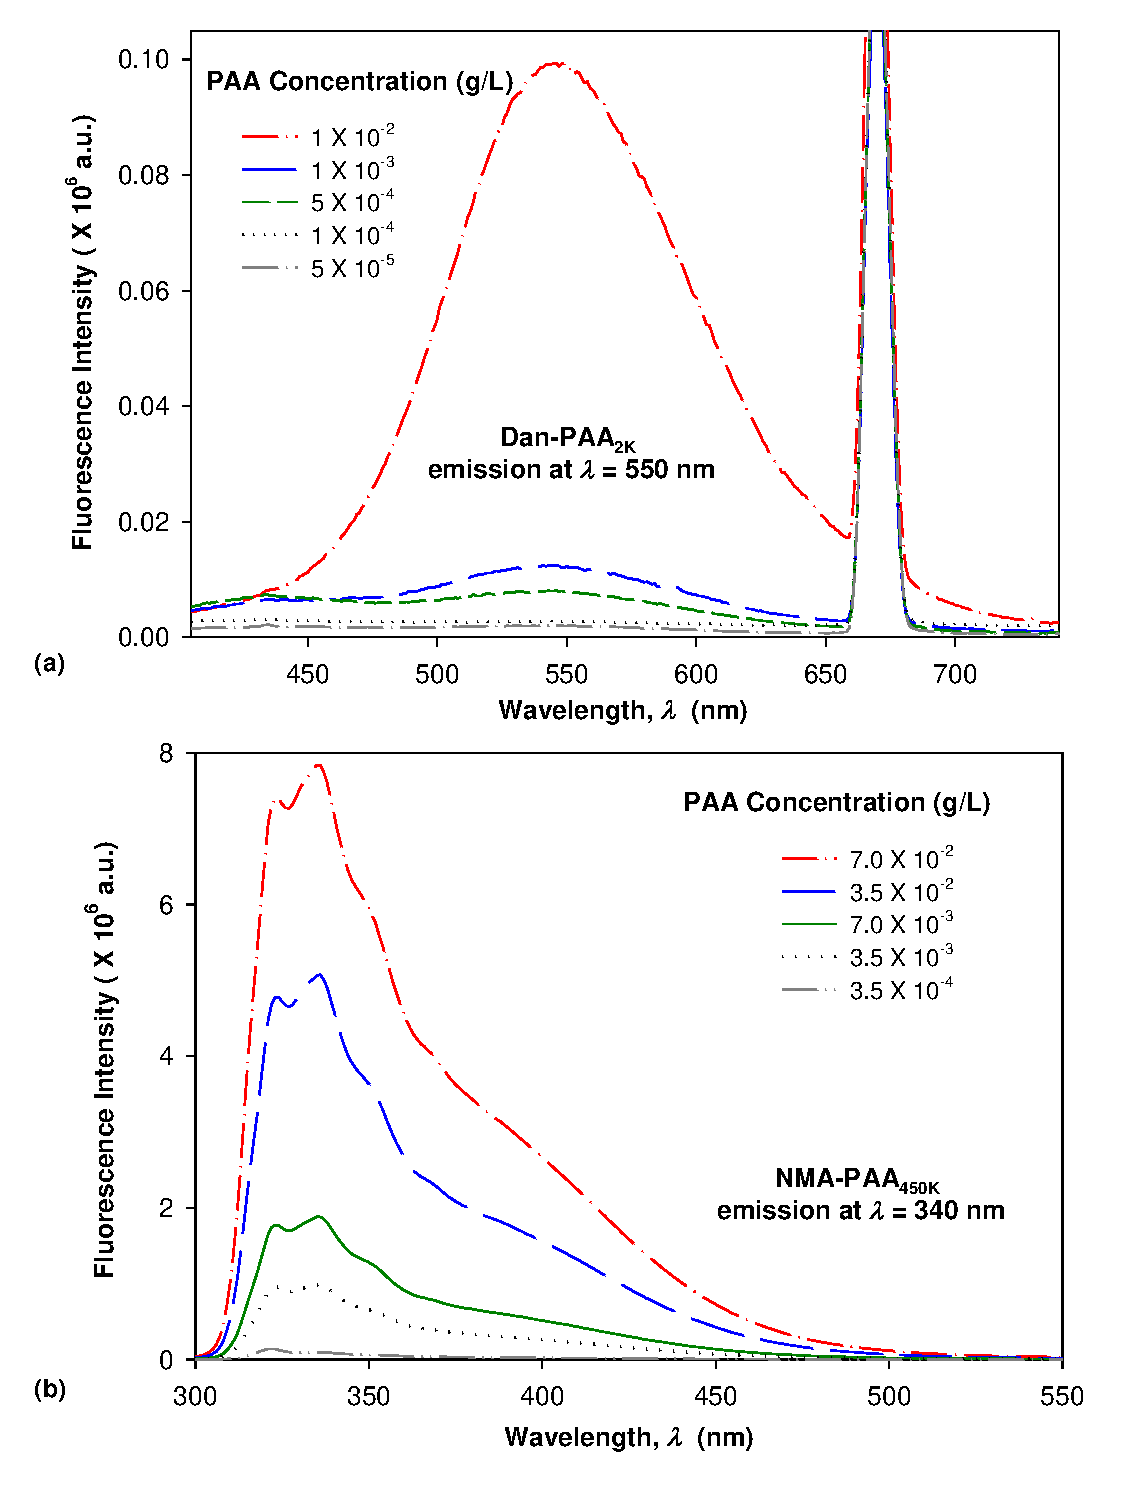
\includegraphics[scale=0.65]{Figure4.pdf}
\caption{Fluorescence emission spectra obtained in
decreasing intensity and corresponding to concentrations from highest to lowest of: a. short-chain labeled PAA (Dan-PAA\textsubscript{2K}), and b. long-chain labeled PAA (NMA-PAA\textsubscript{450K}) in water.}
\label{figure 2}
\end{figure}
 

We compared the fluorescence intensity of the two fluorophore-labeled PAA samples, at the peak maximum.  Although both of the PAA samples were modified by approximately 4\% fluorophores, the fluorescence intensity exhibited by NMA-PAA\textsubscript{450K} was found to be greater by an order of magnitude than that of Dan-PAA\textsubscript{2K} prepared at an identical solution concentration.  The smaller fluorescence signal from the Dan-PAA\textsubscript{2K} is attributed to the dansyl fluorophore, which is known to fluoresce much less intensely in water as compared to nonpolar organic solutions.\cite{weber1954fluorescent,Bednar1985,Chen1983}  A fluorescence signal for both samples, however, was detectable at concentrations above the critical coverage adsorption concentration used for the study ($10^{-4}$ M).  As indicated in Figure \ref{figure 3}, we also determined that there was no significant quenching of one fluorophore by the other, by obtaining the fluorescence spectrum of a mixed sample of both NMA-PAA\textsubscript{450K} and Dan-PAA\textsubscript{2K} in solution at identical concentrations of 5.0 $\times$ $10^{-3}$ g/L (above the coverage concentration).  From Figure \ref{figure 3}, the relative ratio of the NMA-PAA\textsubscript{450K} to Dan-PAA\textsubscript{2K} emission peak in the mixed solution was determined as 13:1.  The relative fluorescence intensity of NMA-PAA\textsubscript{450K} to Dan-PAA\textsubscript{2K} obtained from isolated solutions was similar to that of the mixed PAA solution indicating that the emission of one fluorophore did not perturb the emission of the other by any measurable amount. (Figure \ref{figure 3}).

\begin{figure}[H]
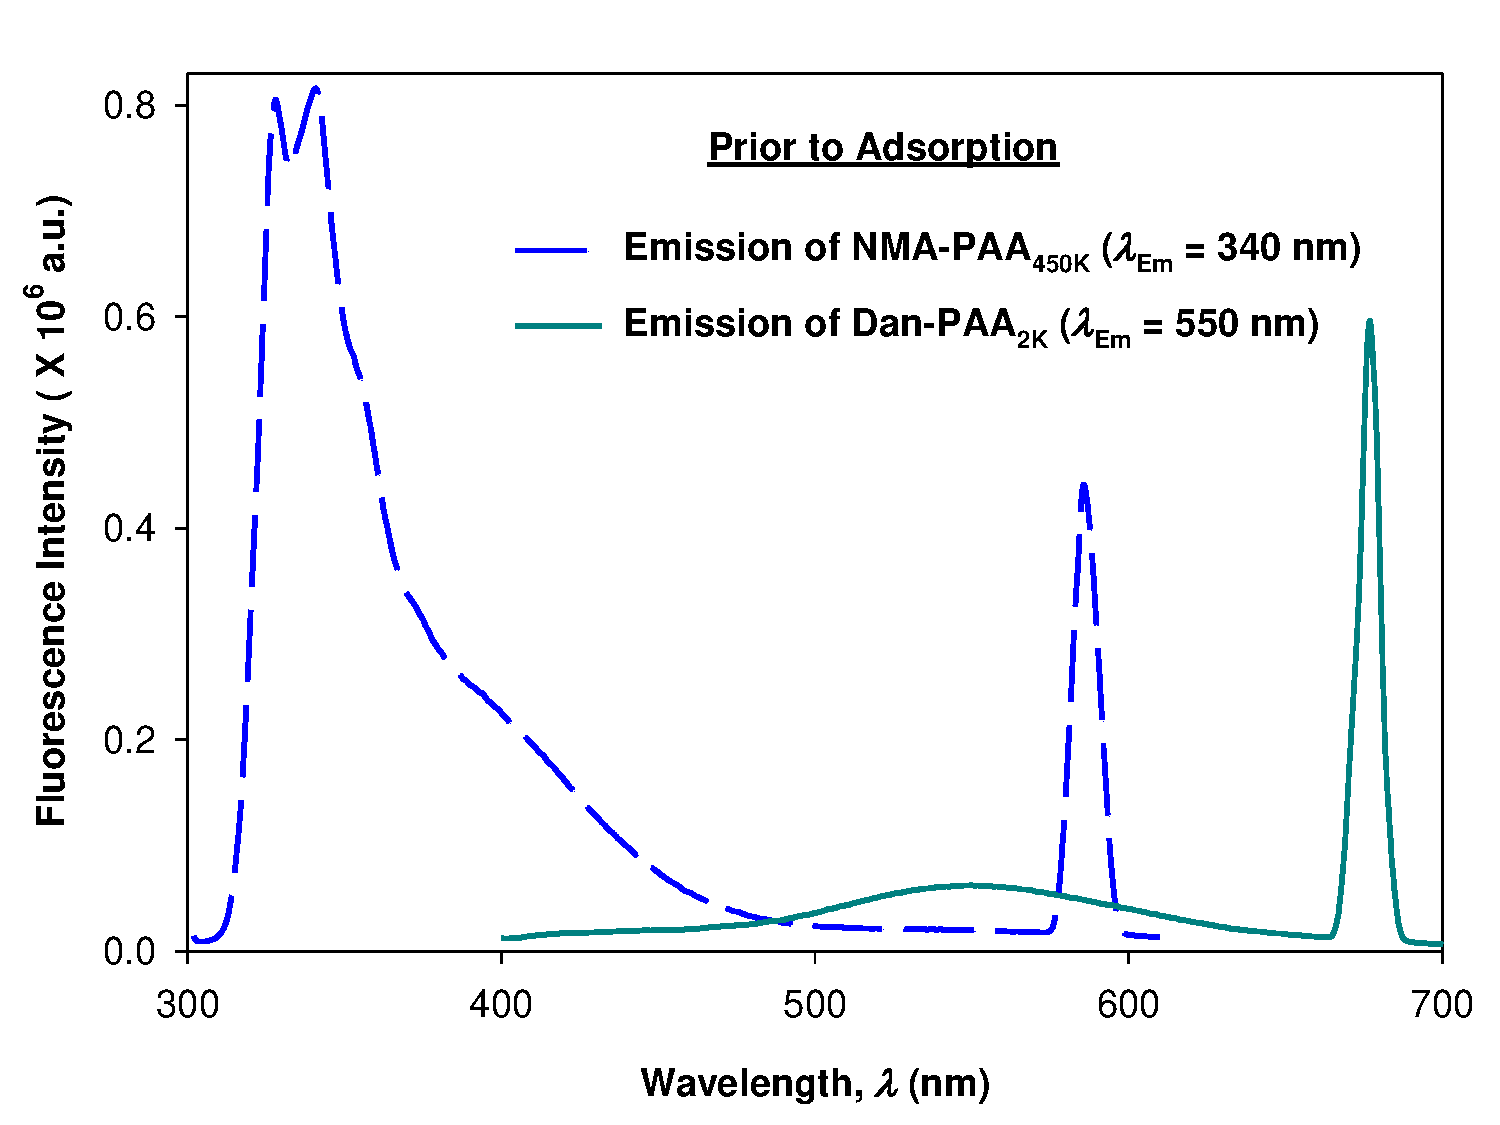
\includegraphics[scale=0.45]{Figure5.pdf}
\caption{Pre-adsorbed fluorescence spectrum of a mixed solution containing $5.0 \times 10^{-3}$ g/L of each of NMA-PAA\textsubscript{450K} (dashed line, $\lambda$\textsubscript{Ex} = 290 nm), and Dan-PAA\textsubscript{2K} (solid line, $\lambda$\textsubscript{Ex} = 335 nm).  Emission intensity ratio of NMA-PAA\textsubscript{450K} to Dan-PAA\textsubscript{2K}  is 13:1.}
\label{figure 3}
\end{figure}

\subsubsection{3.1.2 Competitive Adsorption of Labeled PAA onto a PAH Surface}   %4.1.2
    \label{sec-res-compet}


Successful adsorption of PAA onto a PAH coated surface is known from previous $\zeta$ potential measurements and solid-state NMR spectroscopy of similar multilayer systems.\cite{Burke2003,Smith2004}  We provided an equal surface coverage concentration of both the 2K and the 450K PAA repeat units (number of mers) to a quantitative amount of PAH layered SiO$_2$.  At concentrations lower than that required for complete coverage, both 2K and 450K PAA would adsorb to meet until surface coverage achieved, and such an experiment would fail to test for preferential adsorption.  If experiments are conducted at concentrations higher than that required for surface coverage, we might not observe a significant change in the 
fluorescence signal to identify preferential adsorption. 


Although previous studies examining the preparation of PAH/PAA multilayers suggest adsorption times on the order of tens of minutes, (supplying excess concentration of the adsorbing polyelectrolyte), we allowed 24 h for the competitive adsorption study of PAA since here, we supply only a minimum coverage concentration of short and of long chains of PAA.  After 24 h, we examined the fluorescence of both the PAA/PAH-coated particles (thoroughly rinsed free of excess polymer), and the remaining unadsorbed PAA in the supernatant.  Figure \ref{figure 5} shows the relative fluorescence intensity obtained for the labeled PAA adsorbed on the particles while Figure \ref{figure 6} shows that of the unadsorbed PAA remaining in the supernatant.  After exciting both fluorophores on the particles, no detectable fluorescence emission from Dan-PAA\textsubscript{2K} at $\lambda_{Em}$ = 550 nm was observed.  However, the particles did exhibit a strong emission signal from at $\lambda_{Em}$ = 340 nm.  Similar inspection of the supernatant indicated an opposite trend, where we observed significant fluorescence from Dan-PAA\textsubscript{2K}.  Furthermore the intensity ratio of NMA-PAA\textsubscript{450K}\,:\,Dan-PAA\textsubscript{2K} in the supernatant was 3.4:1, which was significantly less than the original pre-adsorption ratio of 13:1.  Fluorescence analysis of both the PAA adsorbed 
onto the particles and the PAA remaining in the supernatant suggest the preferred adsorption of the higher molecular weight component PAA onto the PAH-coated colloidal particles after 24 hr.  Also, we do not expect the effects of PAA polydispersity to significantly mislead our results since: 1) the two extreme chain lengths differ by two orders of magnitude, and 2) preliminary DLS characterization of the 2K and 450K chains showed negligible overlap in the distribution of their hydrodynamic radius.

\begin{figure}[H]
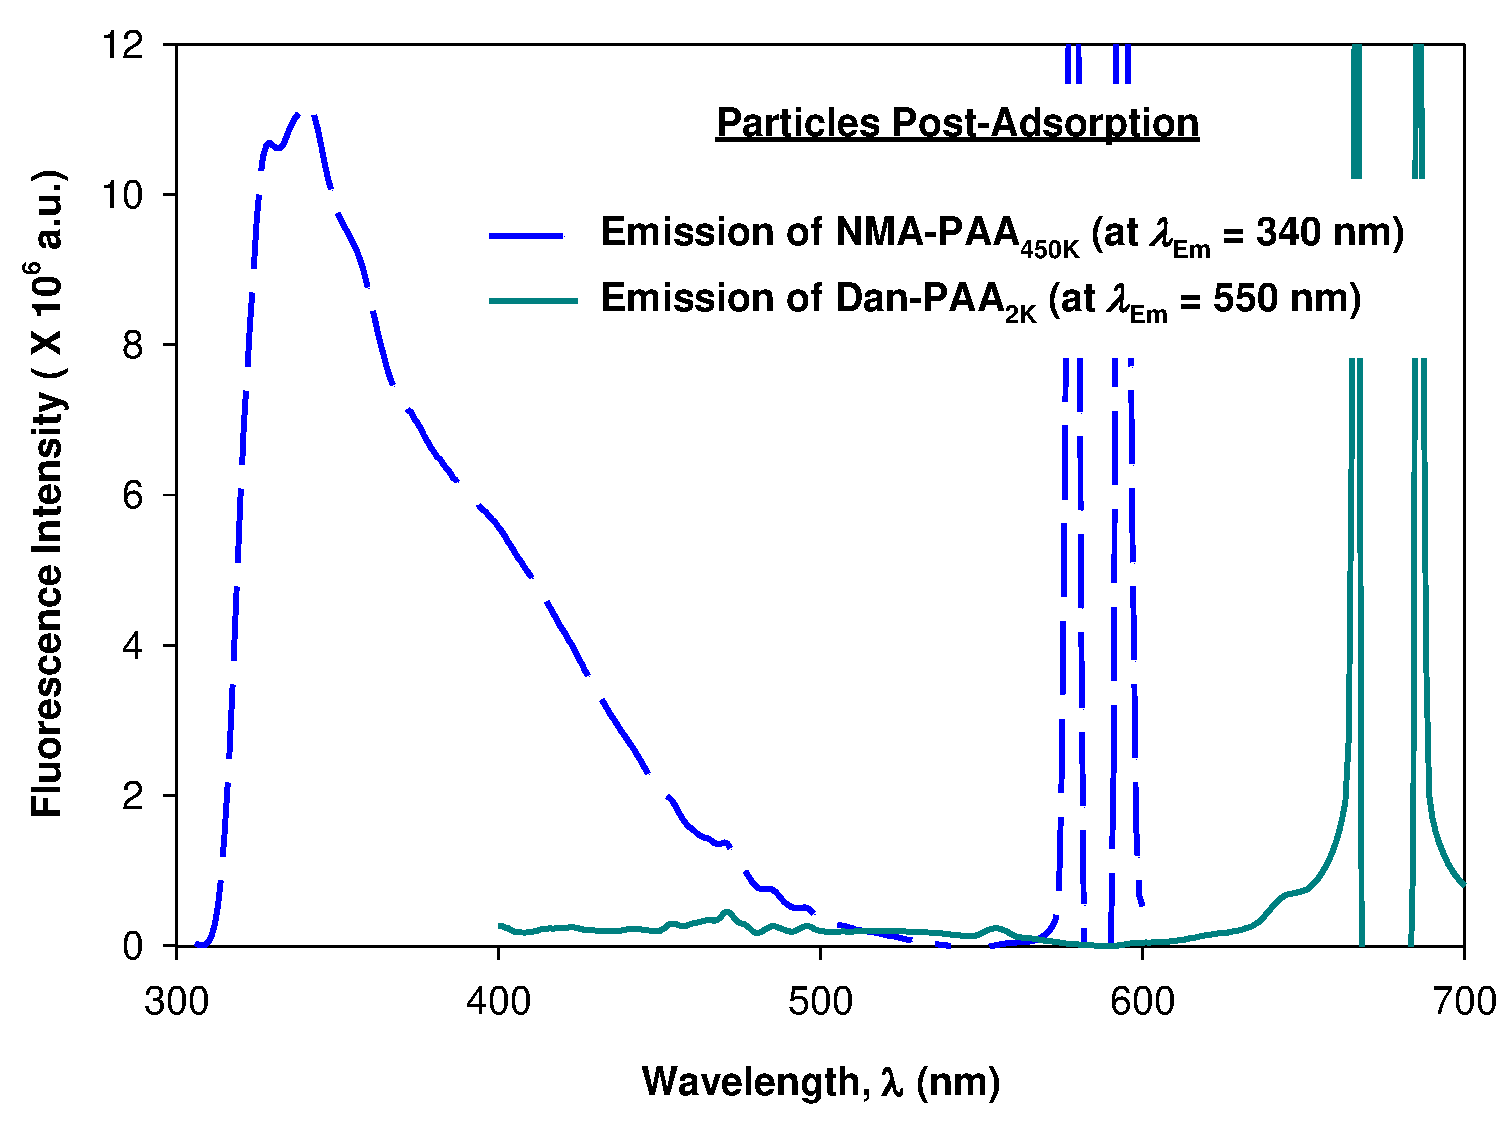
\includegraphics[scale=0.45]{Figure6.pdf}
\caption{Fluorescence emission spectra obtained for variable concentration of: a.\ short-chain labeled PAA (solid line, Dan-PAA\textsubscript{2K}), and b.\ long-chain labeled PAA (dashed line, NMA-PAA\textsubscript{450K}) in water.}
\label{figure 5}
\end{figure}


\begin{figure}[H]
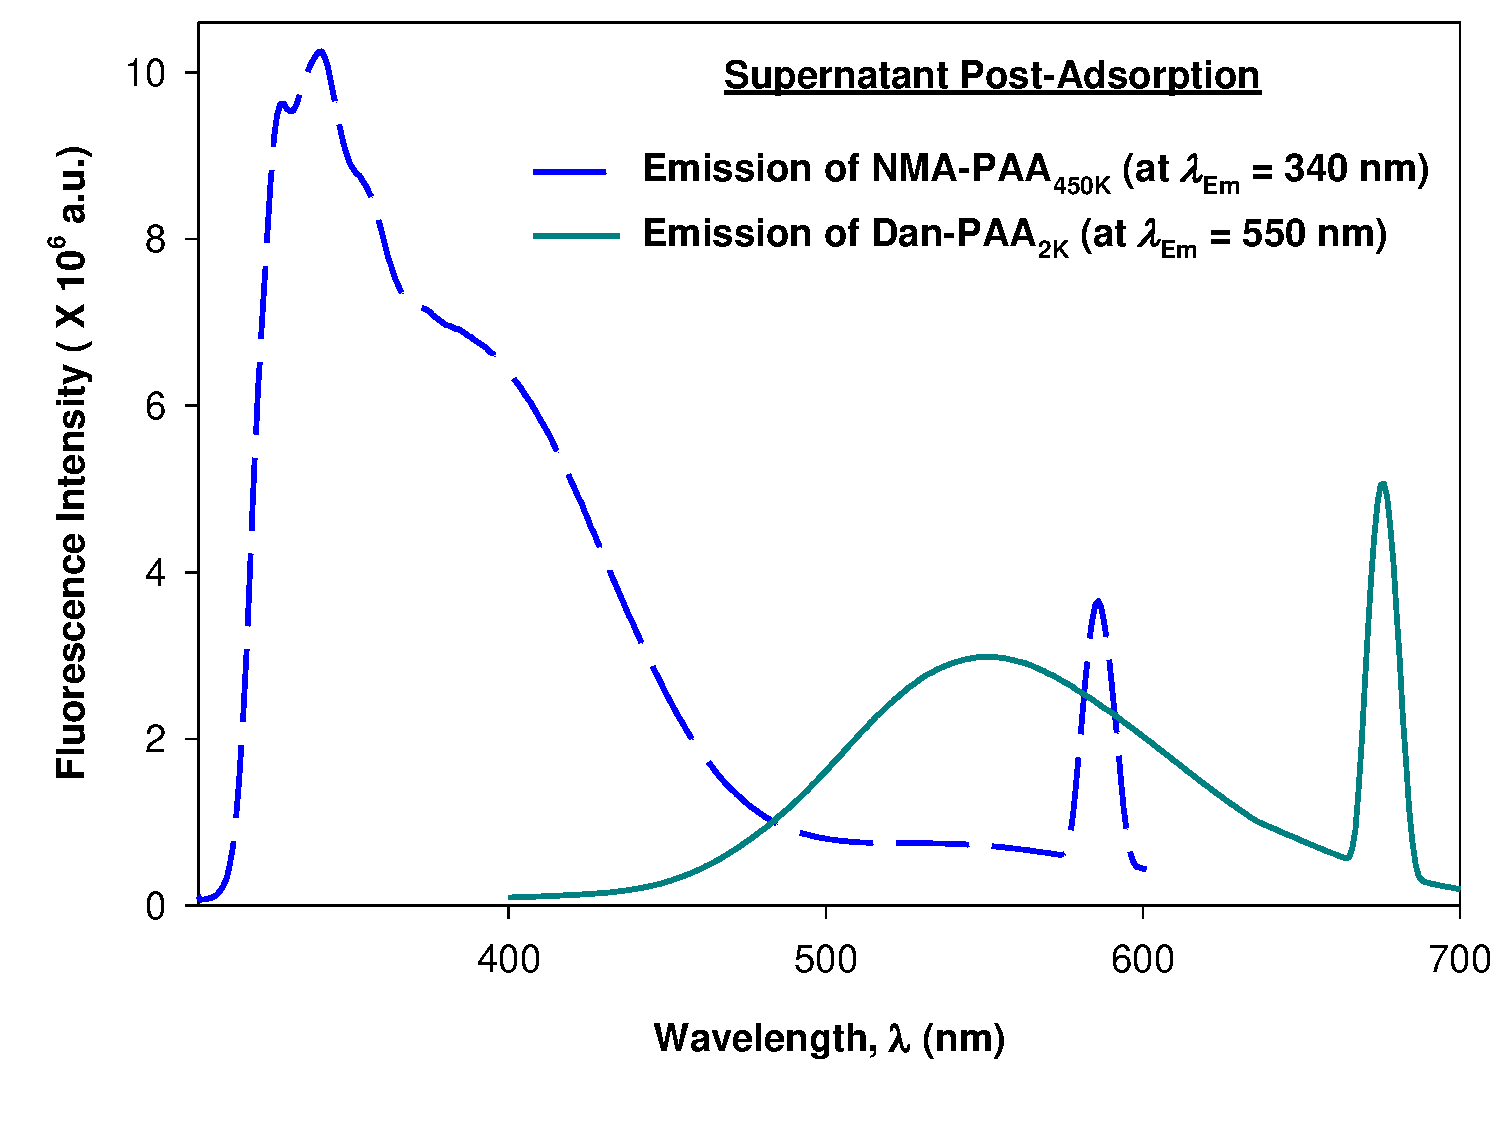
\includegraphics[scale=0.45]{Figure7.pdf}
\caption{Fluorescence emission spectra obtained for variable concentration of: a.\ short-chain labeled PAA (solid line, Dan-PAA\textsubscript{2K}), and b.\ long-chain labeled PAA (dashed line, NMA-PAA\textsubscript{450K}) in water.}
\label{figure 6}
\end{figure}



\subsubsection{3.1.3 General Processes in Adsorption}  %4.1.3
     \label{sec-res-gen}

To understand why there is preferential adsorption of longer chains of PAA onto PAH-coated particles, it is worthwhile to examine the general steps involved in the process of polymer adsorption.  The adsorption mechanism begins by the transport of bulk polymer to the surface-adsorbing site.  Kinetically, this diffusion-limited step would favor the arrival of shorter chains to the surface.  Transport is then followed by polymer attachment to the surface, and lastly rearrangements, which can occur in the adsorbing layer.  The two initial steps generally occur rapidly and the adsorption rate is usually transport-limited since the polymer arriving at the surface adsorbs immediately.\cite{Dijt1990} As surface coverage increases, adsorption becomes hindered.  At this stage, further adsorption is highly dependant on attachment to the remaining free sites.\cite{Hoogeveen1996}  At very high surface coverage and approaching maximum coverage, transport plays a minimal role and the specific attachment process becomes increasingly important.\cite{Hoogeveen1996} Rearrangement processes are also generally much slower and thus some polymer adsorption can be considered to be irreversible at relatively short time-scales.\cite{Cafe1982,Meadows1988}  Therefore, in the case where adsorption is examined at time-scales much larger than that required to achieve full surface coverage, kinetic contributions are less likely to influence the preferential adsorption of polymers and over much longer time-scales.  In this plateau region of an adsorption isotherm adsorption is less dependant on transport.\cite{Hoogeveen1996}



\subsubsection{3.1.4 Polyelectrolyte Adsorption}  %4.1.4
    \label{sec-polyads}

In polyelectrolyte adsorption additional interactions need to be considered which have important thermodynamic implications. The theory of neutral polymer adsorption can be extended to polyelectrolyte adsorption by incorporating Debye-H\"uckel theory.\cite{Chatellier1996}  Polyelectrolytes adsorb onto oppositely charged surfaces when the energy of adsorption exceeds the net entropy resulting from the culmination of entropic losses (associated with the reduction in the number of configurations available to the polyelectrolyte), and entropic gains (associated with the release of counterions).  Whether or not adsorption will occur depends on if there is sufficient energy given to the system to overcome the entropy loss i.e.\ if the temperature is below a critical value to reduce the free energy and to drive towards adsorption.

Enthalpic contributions include the interaction type and strength between the polyion and the surface (i.e.\ electrostatic attraction with each link of the order $k_B$T) as well as the interaction between charged segments (i.e.\ electrostatic repulsion), which oppose adsorption.\cite{Hoogeveen1996,VonGoeler1994}  In the adsorption of charged polymers the surface charge is compensated when the adsorbed charge balances with the surface charge such that the electrostatic attraction of the segments with the surface is balanced by the repulsion of segments in the adsorbing layer.  In polyelectrolyte multilayer adsorption the surface charge is overcompensated, causing net electrostatic repulsion.  In achieving charge overcompensation, weakly charged polyelectrolytes differ from strongly charged polyelectrolytes in that more polyion molecules have to adsorb in order to overcompensate the surface charge and this is why more polyelectrolyte adsorption is generally observed.  Chain stiffness and conformation also have significant effect on adsorption, particularly in the case of weak polyelectrolytes.\cite{Dzubiella2003}  For example, adsorption of weak charged polyelectrolytes onto an oppositely charged surface in the form of “loops and tails” can be favored over a more flat, “train-like” configuration where electrostatic interactions between polyion segments and the surface are maximized. \cite{Borisov1994}  The conformation of polyelectrolyte adsorption is thus highly sensitive to the electrostatic environment during adsorption, for example, the solvent pH and ionic strength.\cite{Notley2004}  In the case of polyelectrolyte multilayer adsorption, nonelectrostatic short range forces such as hydrophobic interactions have also been observed, which enhance stability in adsorption.\cite{Kotov1999}  


\subsubsection{3.1.5 Long- versus Short-Chain Adsorption }  %4.1.5
  \label{sec-longvsshort}

\subsubsection{3.1.5a Enthalpic Considerations}  %4.1.5a
    \label{sec-enthalpic}

In considering the preferential adsorption of PAA onto PAH-coated particles, we assume uniform capping of the SiO$_2$ with the polycation, PAH.  Thus all potential adsorption surface sites are assumed to be entirely composed of PAH repeat units, and the adsorption occurs on a chemically homogeneous surface.  This is a reasonable assumption for PAH adsorbed in excess concentration and under solution conditions that render it a weakly charged polycation (i.e.\ adsorption solution adjusted to pH = 9, near the pK of PAH).\cite{Burke2003,Smith2003}  This implies that all electrostatic attractions between identical polycations and polyanions are energetically equivalent (i.e.\ of equivalent $k_B$T, since in both cases each PAA sample contains an equal number of repeat units).\cite{Dubas1999}  Additionally, the enthaplic loss derived from displacement of counterions from their associated polyelectrolytes is also similar for the short and long chain systems.  Hence, if we assume that the electrostatics is one of the dominant driving forces in multilayer formation, we can simplify the thermodynamic comparison by presenting an ideal case in which the enthalpic energy is identical in the two cases, under identical solvent conditions (i.e.\ pH value and ionic strength). 

Interestingly, the addition of a high concentration of electrolyte has been shown to influence the adsorption of polyelectrolytes of varying chain lengths.  In previous adsorption studies of a strongly charged polyelectrolyte, poly(styrene sulfonate) onto a chemically homogeneous Fe$_2$O$_3$ surface, preferential adsorption was observed for shorter chains from a salt-free solution while longer chains were preferred in the presence of 0.1 M NaCl.\cite{Ramachandran1987,Ramachandran1988}  Adsorption studies of PAA,\cite{Wright1987} polyacrylate,\cite{Bain1982} and carboxymethyl cellulose\cite{Bain1982} adsorbed onto BaSO$_4$ report similar preferential adsorption of low molecular weight components in the absence of salt.  However, these adsorption isotherms reveal significant displacement of the low molecular weight with the high molecular weight in the presence of 0.5 M NaCl.\cite{Bain1982} This adsorption behavior is rationalized using a sequential adsorption process, which suggests that first, smaller chains are adsorbed.\cite{DeLaat1995}  For example, short PAA chains initially adsorbed eventually generate an electrostatic barrier from charge overcompensation occurring on the positive surface.  This barrier strongly affects the diffusion of chains towards the PAA covered surface.  Specifically, the barrier can prevent longer chains from accessing the surface, and thus limits their displacement of pre-adsorbed shorter chains.  With an increased salt concentration the barrier is lowered, permitting longer chains to reach the surface and adsorb.  At this point, the adsorption preference is shifted to longer chains as experimentally observed.\cite{DeLaat1995}  We therefore suggest that our observation of preferred adsorption of longer PAA chains onto PAH after a 24 h adsorption period is likely restricted to the time-window past which such displacement effects are likely to occur.  Further supporting evidence for the occurrence of short-chain displacement is given by recent adsorption experiments of model cationic oligomers onto colloids,\cite{Shin2001} and short polyions assembled onto proteins,\cite{Houska2004} which suggest that shorter chains have more difficulty forming loops and tails under assembly conditions where the polyion is weakly ionized.  As such, adsorbed short-chain polyions can be more easily displaced by longer chains from failure to make a sufficient number of ionic contacts.  

\subsubsection{3.1.5b Entropic Considerations}  %4.1.5b
    \label{sec-entropic}

Although the LBL self-assembly technique is based on electrostatic attraction of positively and negatively charged polyions, the primary driving force is presumed to be entropy and not enthalpy.  In the electrostatic assembly of multilayers, the condensation of oppositely charged polyions liberates low molar mass counterions.  This process increases the entropy of the system, comparable to the polyelectrolyte complexes formed in solution.\cite{Kabanov1994,Philipp1989}  Thus, although other interactions such as hydrophobic interactions, charge transfer interactions, $\pi{-}\pi$ stacking forces, or H-bonding may also contribute, the successful formation of polyelectrolyte multilayers is primarily attributed to the entropy gain from ion 
exchange.\cite{Kotov1999,Bertrand2000}  

In determining the effect of entropy on the preferential adsorption of short versus long chains of polyelectrolytes, three entropic contributions need to be considered.  First is the net entropy associated with the liberation of the counterions.  Since we provide an identical number of repeat units for both long- and short-chain PAA, and assume coverage adsorption in both cases, the counterion release entropy should be similar for both 2K and 450K.  Secondly, we need to compare the configurational entropy of the short- versus long-chain polyelectrolyte upon adsorption.  As the polyelectrolyte chain length is increased, the entropy penalty associated with the adsorption becomes greater.  This is because there are more configurational restrictions to surface-bound long chains as compared to adsorbed short chains.  The loss in configurational entropy upon adsorption is therefore expected to be much larger for the 450K PAA, which would favor short-chain adsorption.  Lastly, we need to compare the configurational entropy of the free polyelectrolytes in solution.  There is a far greater entropic gain from having more shorter chains in solution, which can explore a greater number of configurational states than a fewer longer chain species in solution.  Similar to the liberation of counterions which drives the LBL assembly process, the entropy gain of having more free short chains in solution favors the preferential adsorption of long-chain PAA onto the PAH surface.  Experimentally, the configurational entropy difference between short and long-chains of PAA in solution appears to be the governing factor leading to the preferential adsorption of 450K PAA.  Moreover, this argument is supported by reports of shorter-chain polyelectrolyte displacement in exchange for adsorption of longer-chains on Fe$_2$O$_3$ and BaSO$_4$ in the presence of salt, as previously mentioned.\cite{DeLaat1995}  Analysis of both the fluorescence spectrum of the PAA-adsorbed particles, and that of the remaining supernatant after the adsorption, suggest that the preferential adsorption of long- over short-chain PAA is dominated by the entropy gain of keeping short chains free in solution.

\subsection{3.2  Theoretical Validation: Model Comparison to Experimental Results}    %4.2
    \label{sec-res-theor}

To validate our experimental results, 
we compare the data to the numerical predictions of our mean field lattice model.
The following, Table 1 gives the numerical values that we use for the key parameters in our model.
These values were chosen to be consistent with 
2 g/L of colloidal SiO$_2$ spheres having diameter 85 nm, and having distance between neighboring lattice sites equal to bond length of 0.4 nm between mers.

\begin{table}
\begin{center}
\begin{tabular}{|c|c|c|}
    \hline
     Variable & Description  & Value   \\ \hline\hline
     %**SK** 6250??
    $\leng_L$ &  mers in a long chain &  6250 \\  
    $\leng_S$ & mers in a short chain &28  \\
    $n$ & $\leng_L/\leng_S$  &   231  \\
    $n_L$ & number of $\leng_L$-mers & 206  \\
    $n_S$  & number of $\leng_S$-mers & 5562  \\
    $q$   & surface coordination number & 4  \\
    $V_{latt}$  & sites in model volume & $6.6\times          10^{9}$\\
    $S_{latt}$  & sites on surface of sphere  & 143750  \\
    $a$  & max number of long chains on surface & 23 \\
      \hline
\end{tabular}
\end{center}
\caption*{\textbf{Table 1: Numerical Parameters Based on Experiment}}
\end{table}

The results of our model are shown in Figure \ref{figure 11}, which demonstrates the decreasing behavior of the ratio of probabilities 
$\left(\frac{|\mathcal{E}_{j+1}|}{|\mathcal{E}_j|}\right)$ as a function of the number $j$ of $\leng_L$-mers (long-chains) adsorbed to the colloid surface (see Supporting Material section 1.2). We observe that the ratio of probabilities are all much greater than one, corresponding to $|\mathcal{E}_j|$ increasing rapidly as $j$ increases. That is, as we increase the number of long chains (and decrease the number of short chains) bound to the colloid surface, the corresponding number of model configurations increases rapidly.  (Recall that a model configuration includes arrangements of unattached chains in solution as well as of adsorbed chains). This implies that the system has a preference for full coverage of the colloid surface by as many $\leng_L$-mers (long-chains) as possible, i.e.\ that the probability of $\mathcal{E}_a$ (i.e.\ $\mathcal{E}_{23}$) is greater than for any other $\mathcal{E}_j$.  


\begin{figure}[H]
\centering
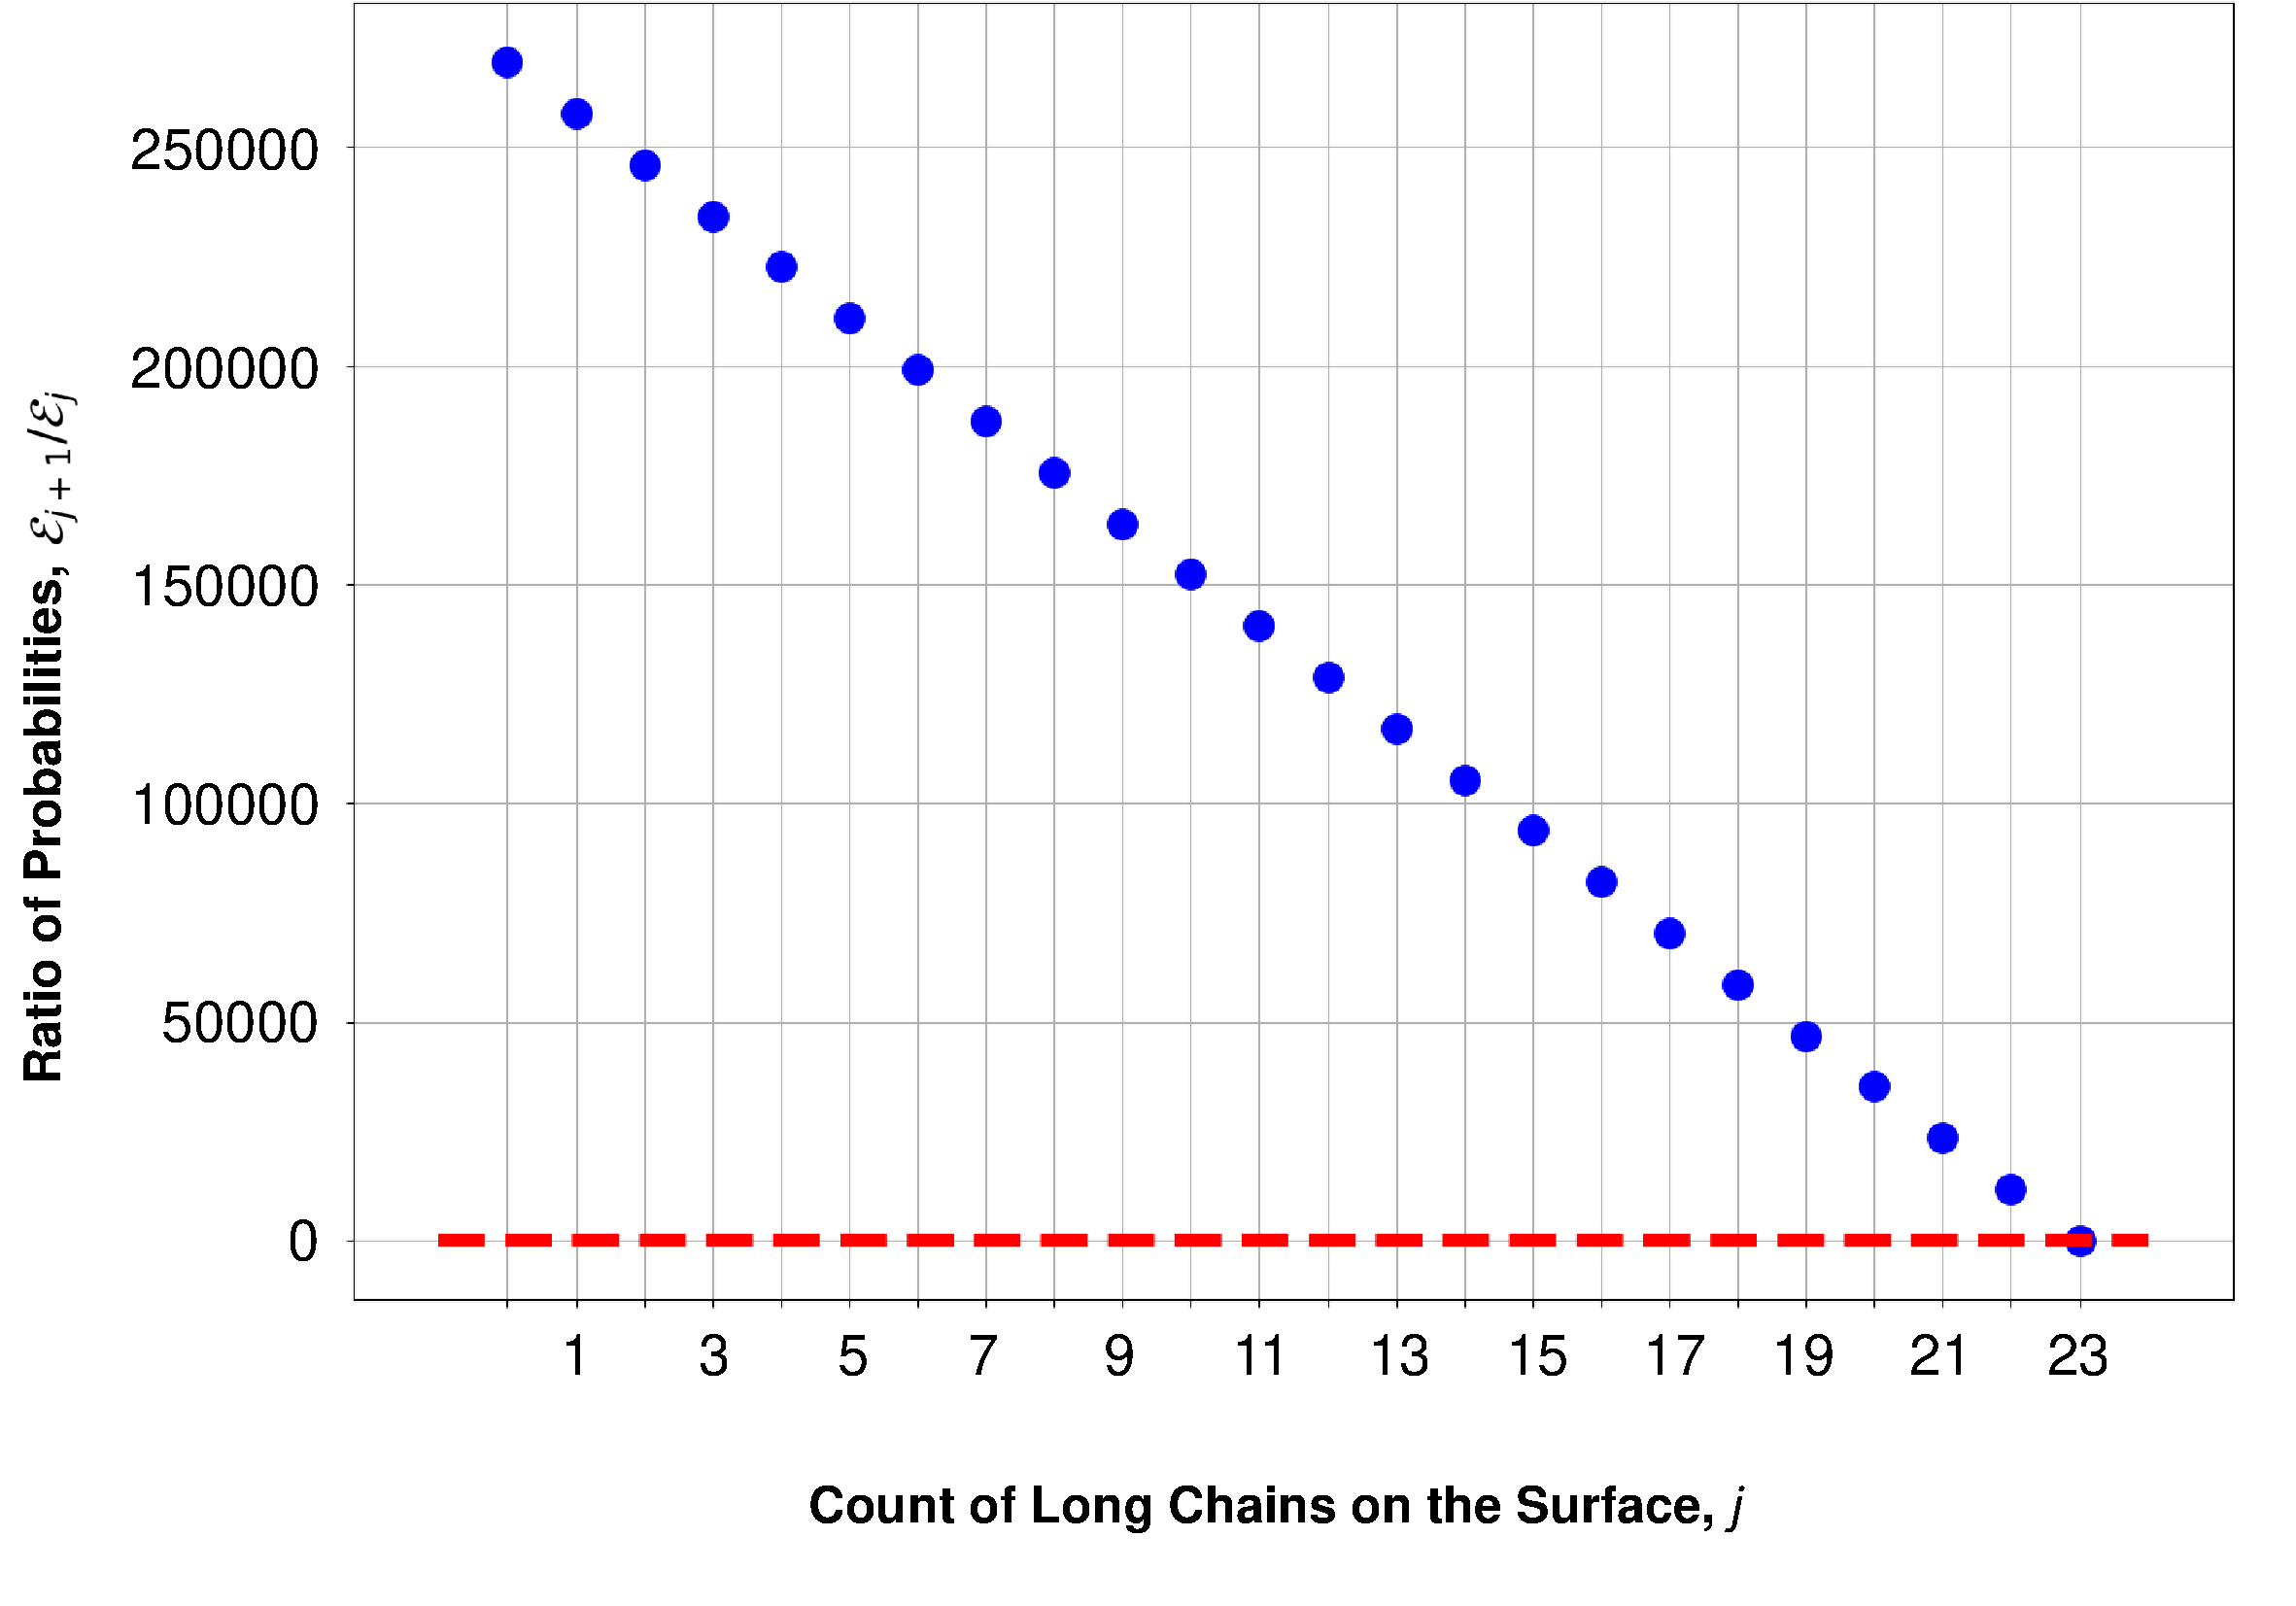
\includegraphics[scale=0.35]{Figure8.pdf}
\caption{We find the value of $j$ (number of long chains on the surface) corresponding to the two consecutive attachment scenarios whose ratio $\frac{|\mathcal{E}_{j+1}|}{|\mathcal{E}_j|}$ (dots) is equal to one (dashed line), which indicates a plateau (or optimal point) of the underlying function $|\mathcal{E}_j|$. This implies that the algorithm iterating through the attachment scenarios has located a preferential scenario for that specific count of long chains on the surface, $j$.}
\label{figure 11}
\end{figure}

Equation (\ref{eq.jstar}) says that the likeliest fraction of the colloid sphere's surface that is covered by short polymers ($1-\frac{j^*}{a}$) is approximately proportional to the concentration of monomers corresponding to those appearing in short chains only
($n_s\,\leng_L/V_{latt}$).  The latter quantity is $3\times 10^{-6}$ when we use the above tabulated values, implying negligible coverage of the surface by short chains.  In particular, the formula of equation (\ref{eq.jstar}) tells us that the most likely value of $j$ is $j^*\approx 22.99$, which is consistent with the value $a=23$ (maximum possible coverage by long chains).

To summarize, our model calculations show that the ratio of probabilities $|\mathcal{E}_{j+1}|/|\mathcal{E}_j|$, related to the Boltzmann configurational entropy (see Supporting Material section 1.3), drives preferential adsorption of long chains on the surface over short. This result is consistent with experimental observations.

\section{4. Conclusions}
   \label{sec-conc}

We have studied competitive adsorption of short- (2K) vs.\ long- (450K) chain PAA polyelectrolyte macromolecules onto PAH coated silica spheres in aqueous solution. Observed both experimentally with optical fluorescence spectroscopy, and theoretically by a mean field lattice model, long-chains where preferentially adsorbed onto the surface when presented with an equal number of mers, while short chains preferred to reside in solution. This is rationalized and theoretically verified as due to a favorable gain in configurational entropy of long-chains at the surface in equilibrium. This study provides insights on entropy driven chain-length dependence in layer-by-layer assembly of polyelectrolyte multilayer surfaces and defines an important advancement in the development of a mathematical framework for directing adsorption behavior and surface properties. Such insights on polyelectrolyte adsorption behavior and modeling will enable optimization of future industrial processes for developments of polyelectrolyte membranes, biomedical coatings, and applications in surface modification.

\section{Acknowledgments}
We gratefully acknowledge funding by the Natural 
Sciences and Engineering Research Council of Canada.
C.B. is grateful to York University for hosting his sabbatical leave, to work in the BioPhysics Group there led by Prof.\ Mermut.

\section{Supporting Information Available}
1.  Calculations for the Mean-field Lattice Model, 
including: 1.1 Estimating the Number of Configurations;
1.2 Interpretations about $\mathcal{E}_j$ from 
ratio $|\mathcal{E}_{j+1}|/|\mathcal{E}_j|$;
1.3 Derivation of the Boltzmann Entropy from the 
Ratio Approximation.  This material is available free of
charge via the internet at  http://pubs.acs.org

\bibliography{LongShort}

\end{document}